%----------------------------------------
\section{Supervised Machine Learning: Regression and Classification}
%----------------------------------------

This foundational course established the core principles of machine learning. It provided a comprehensive journey from the mathematical formulation of learning problems to the implementation of gradient-based optimization for both continuous (regression) and discrete (classification) prediction tasks.

\begin{figure}[H]
    \centering
    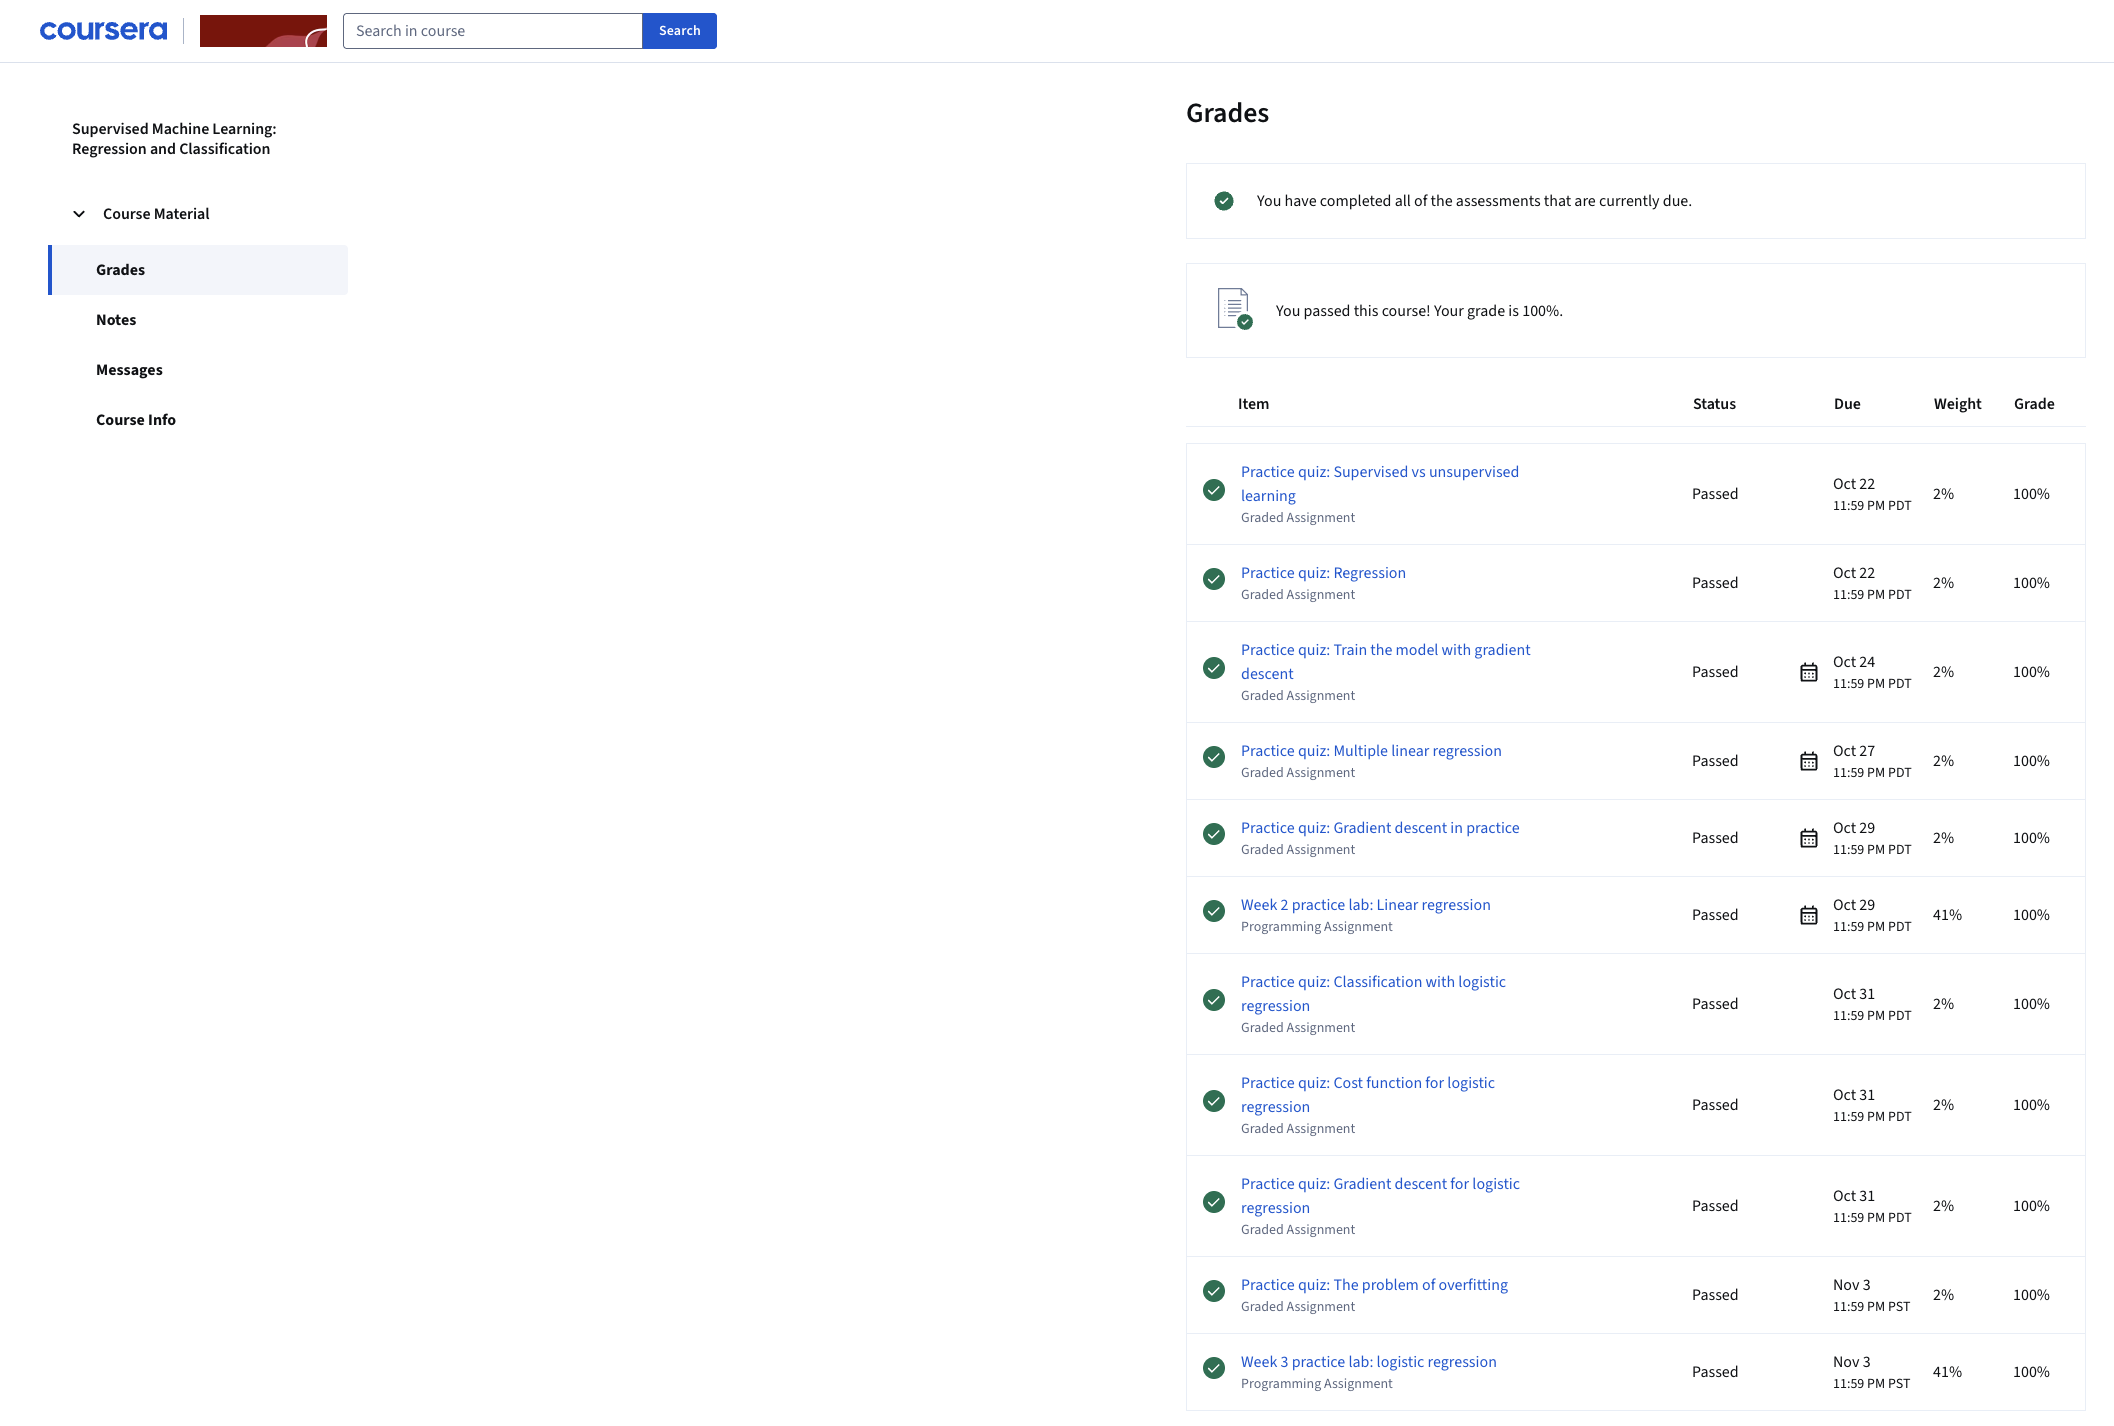
\includegraphics[scale=0.5]{Image/c1.png}
    \caption{Course 1 completed}
\end{figure}

%----------------------------------------
\subsection{Week 1: Introduction to Machine Learning}
%----------------------------------------

\subsubsection{Key Insights and Learnings}

This module introduced the fundamental paradigm shift from traditional programming to data-driven learning.

\begin{itemize}
    \item \textbf{The Supervised Learning Framework:} Structured the problem-solving approach around three core components:
    \begin{enumerate}
        \item \textbf{Model Representation:} Mathematically defined the relationship between inputs $x$ and output $y$ (e.g., Linear Regression $f_{w,b}(x) = wx + b$).
        \item \textbf{Cost Function ($J$):} Quantified the model's error. For regression, the \textbf{Mean Squared Error (MSE)} is used to measure the average squared difference between predictions and actual targets.
        \item \textbf{Gradient Descent Optimization:} Implemented an iterative algorithm that updates parameters ($w, b$) by moving against the gradient of the cost function ($\alpha \frac{\partial J}{\partial w}$) to reach the global minimum.
    \end{enumerate}

    \item \textbf{Learning Paradigms:}
    \begin{itemize}
        \item \textbf{Supervised Learning:} Training models on labeled data (Input $X$ $\rightarrow$ Output $Y$) to predict future outcomes.
        \item \textbf{Unsupervised Learning:} Extracting hidden structures or clusters from unlabeled data (explored deeply in later courses).
    \end{itemize}
\end{itemize}

\subsubsection{Learning Evidence}
\begin{figure}[H]
    \centering
    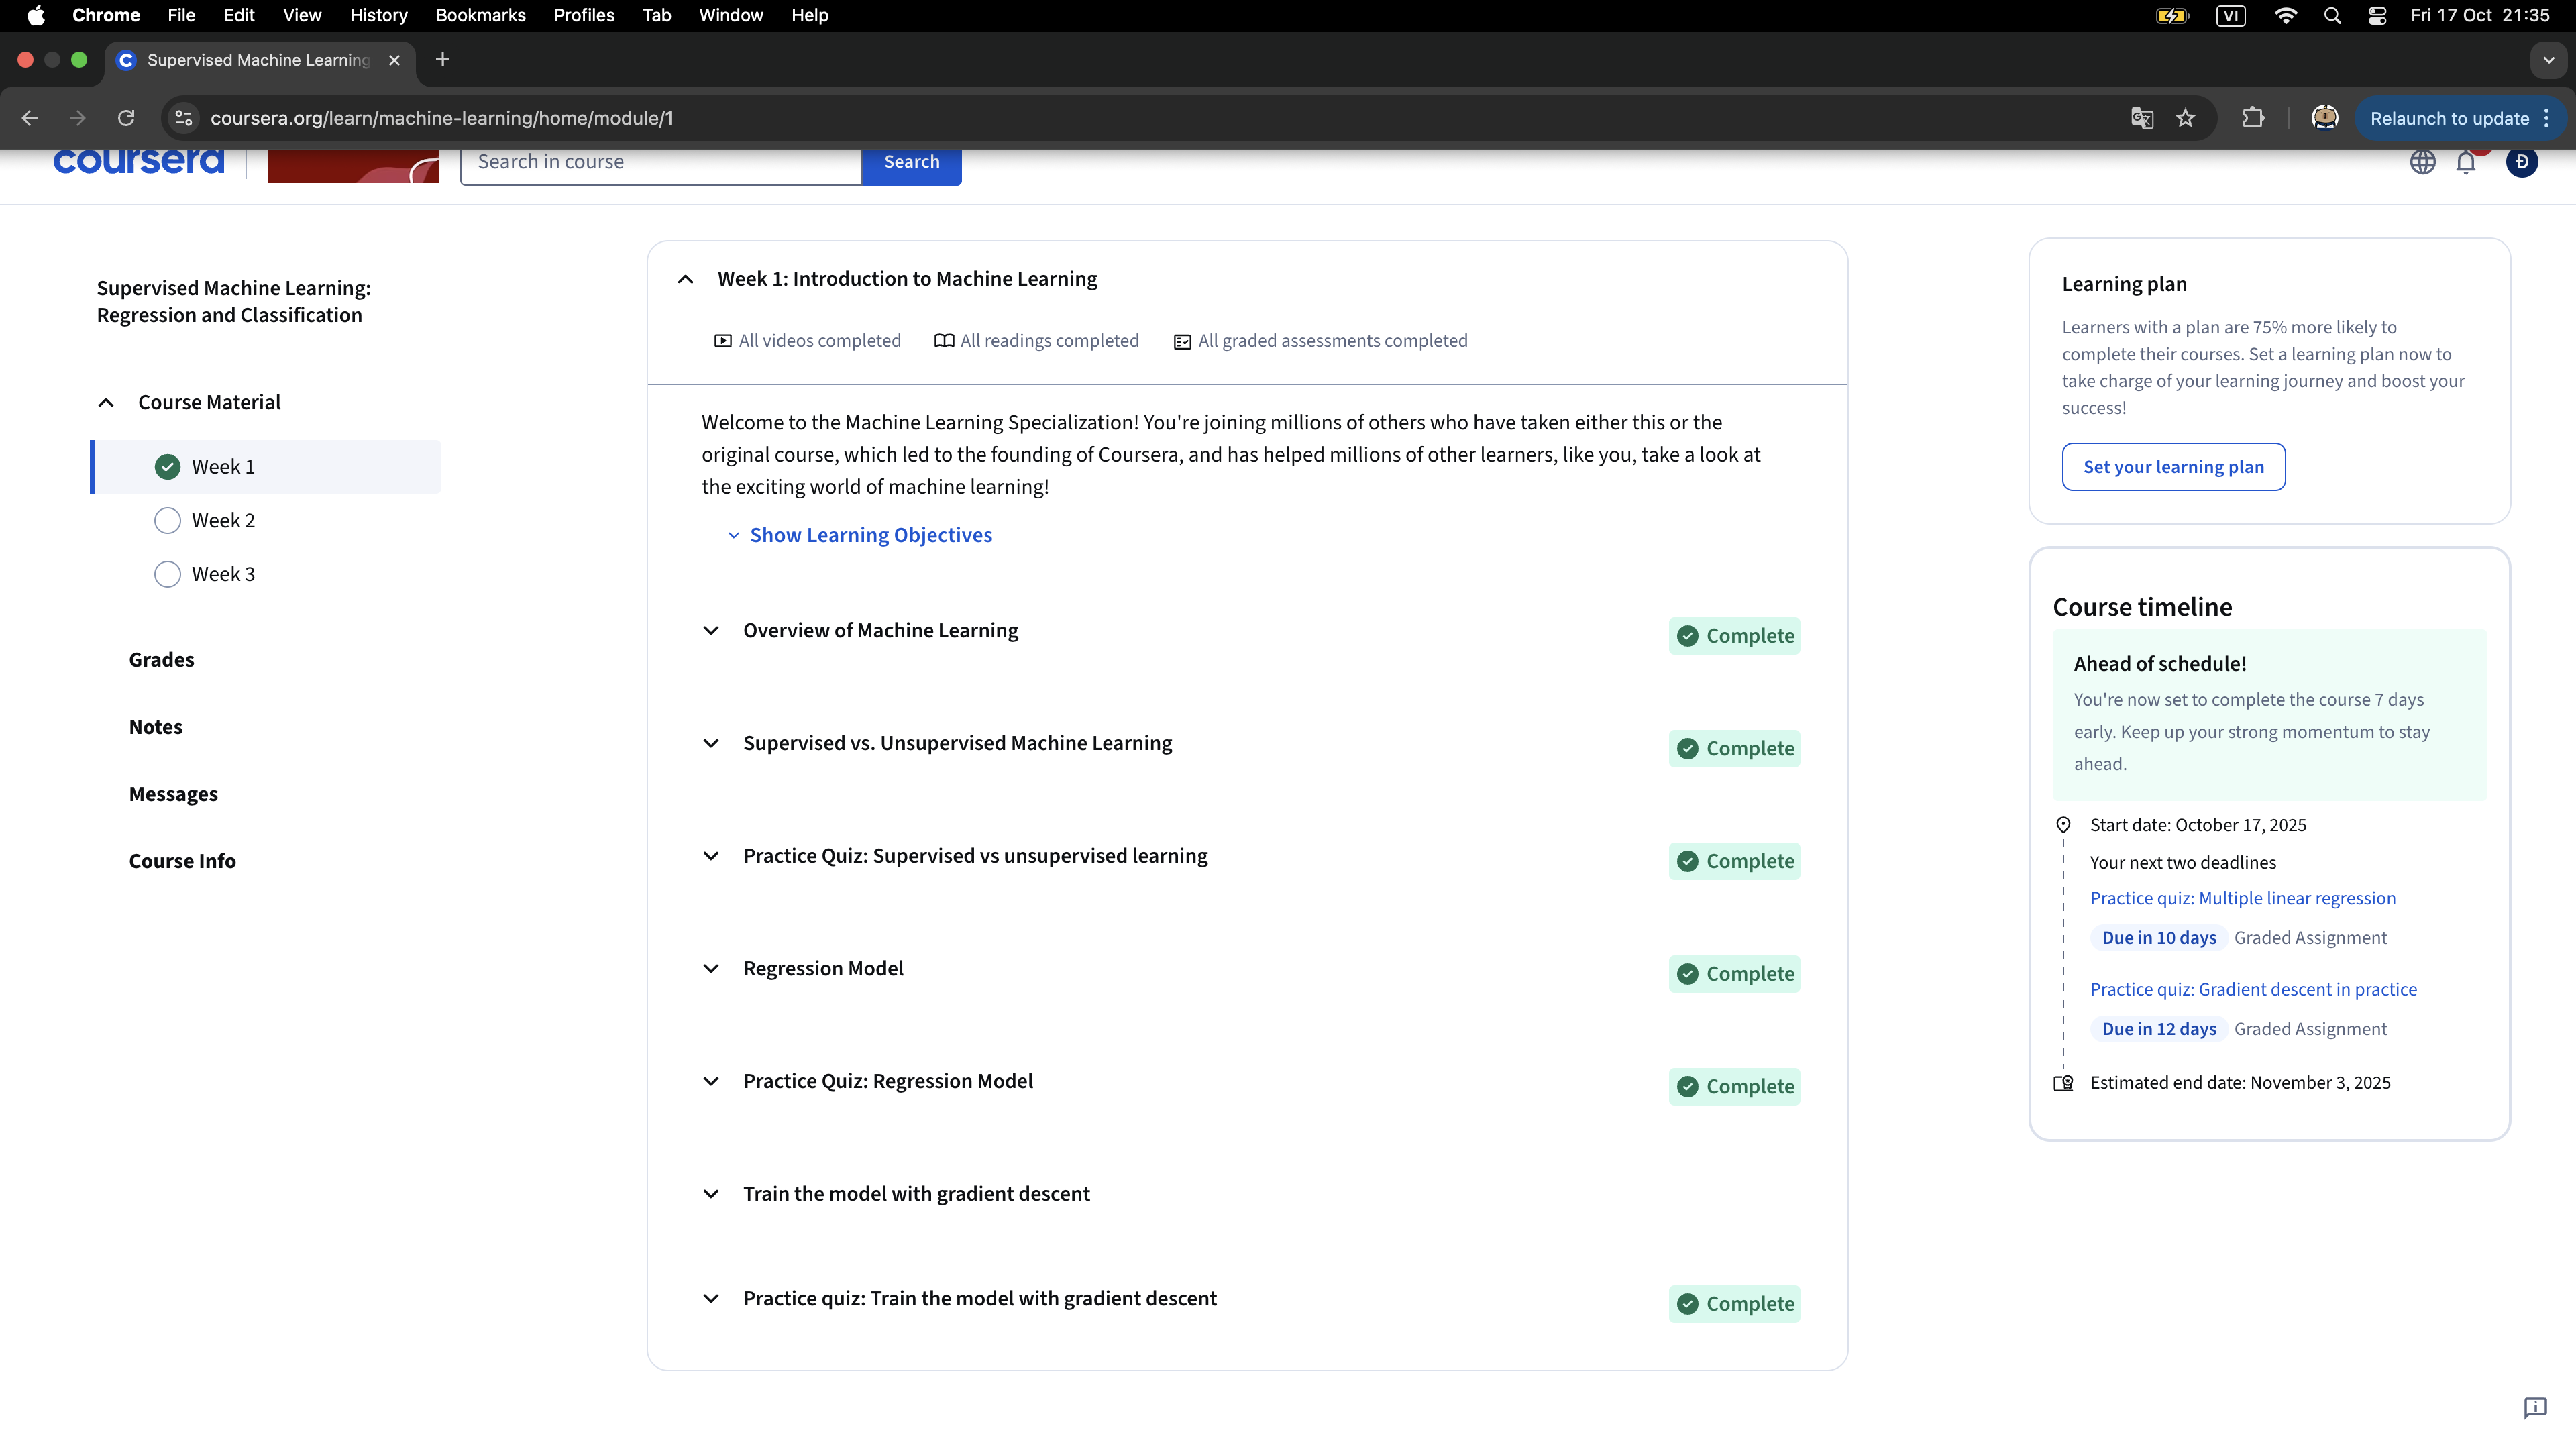
\includegraphics[scale=0.25]{Image/c1_w1.png}
    \caption{Lesson's completed date (17/10/2025)}
\end{figure}

\subsubsection{Graded Assignment Evidence}
\begin{figure}[H]
    \centering
    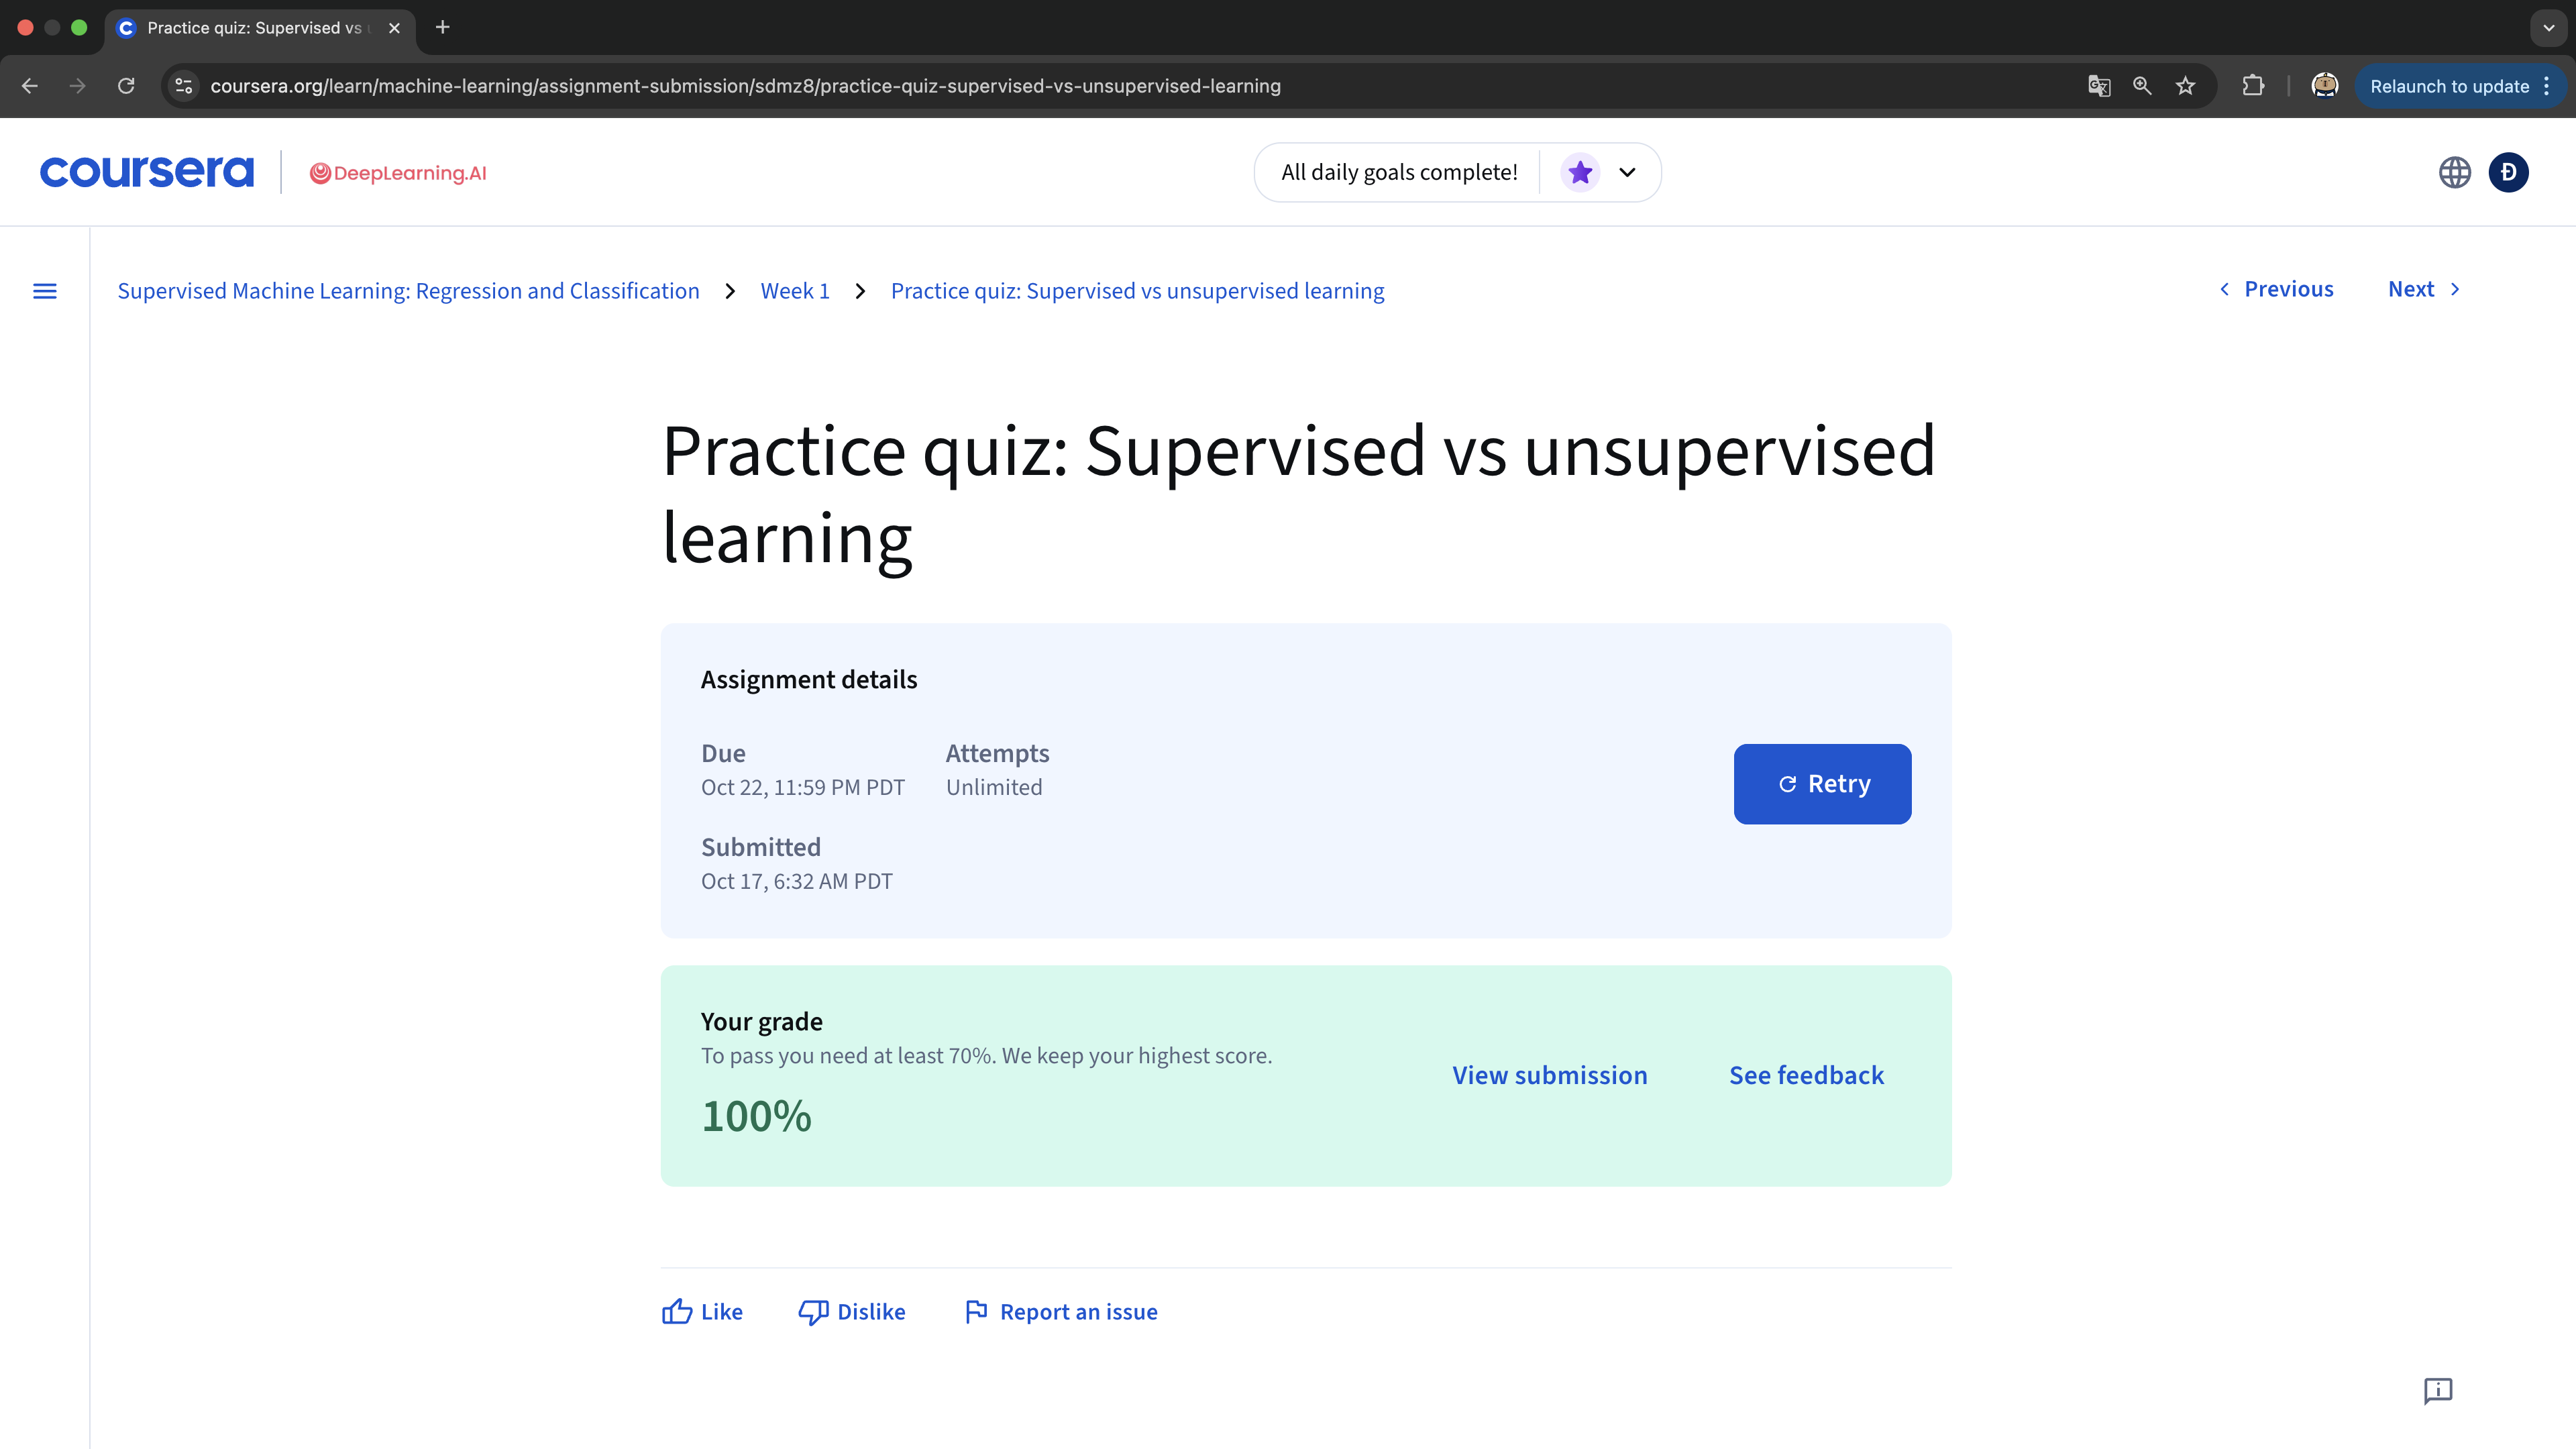
\includegraphics[scale=0.25]{Image/c1_w1_q1.png}
    \caption{Completed Graded Assignment 1 (Supervised vs unsupervised learning)}
\end{figure}

\begin{figure}[H]
    \centering
    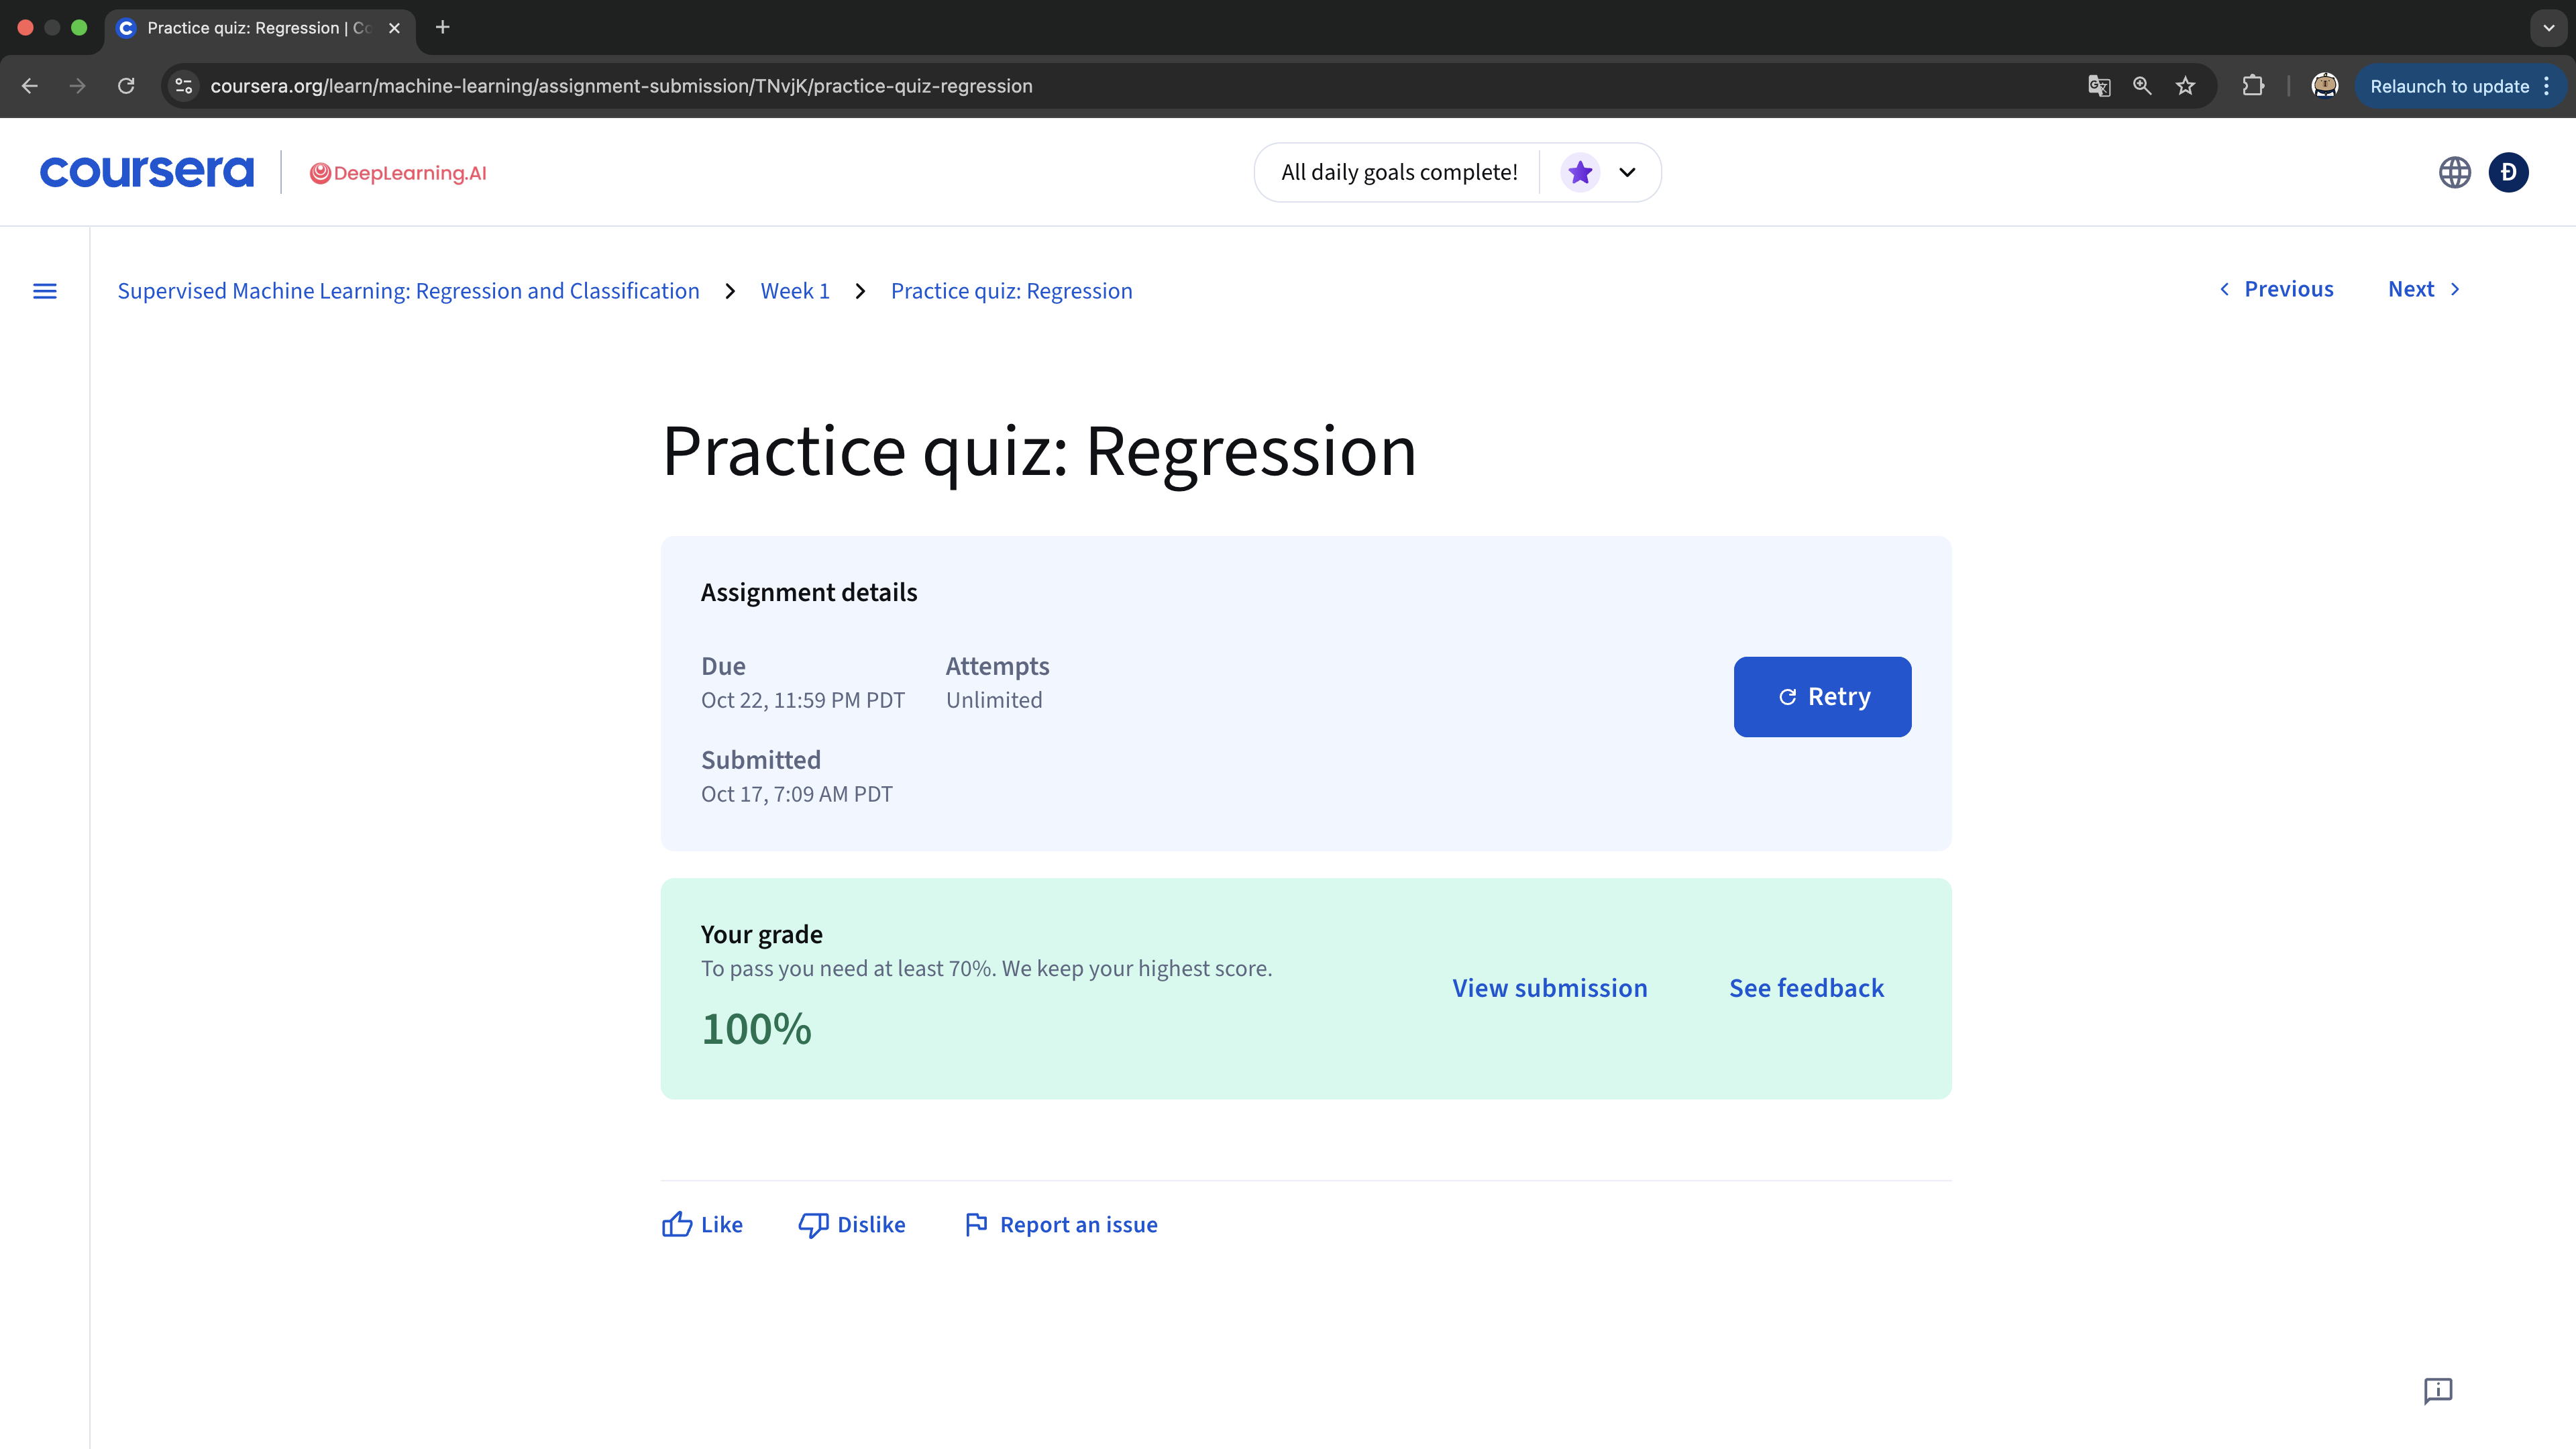
\includegraphics[scale=0.25]{Image/c1_w1_q2.png}
    \caption{Completed Graded Assignment 2 (Regression)}
\end{figure}

\begin{figure}[H]
    \centering
    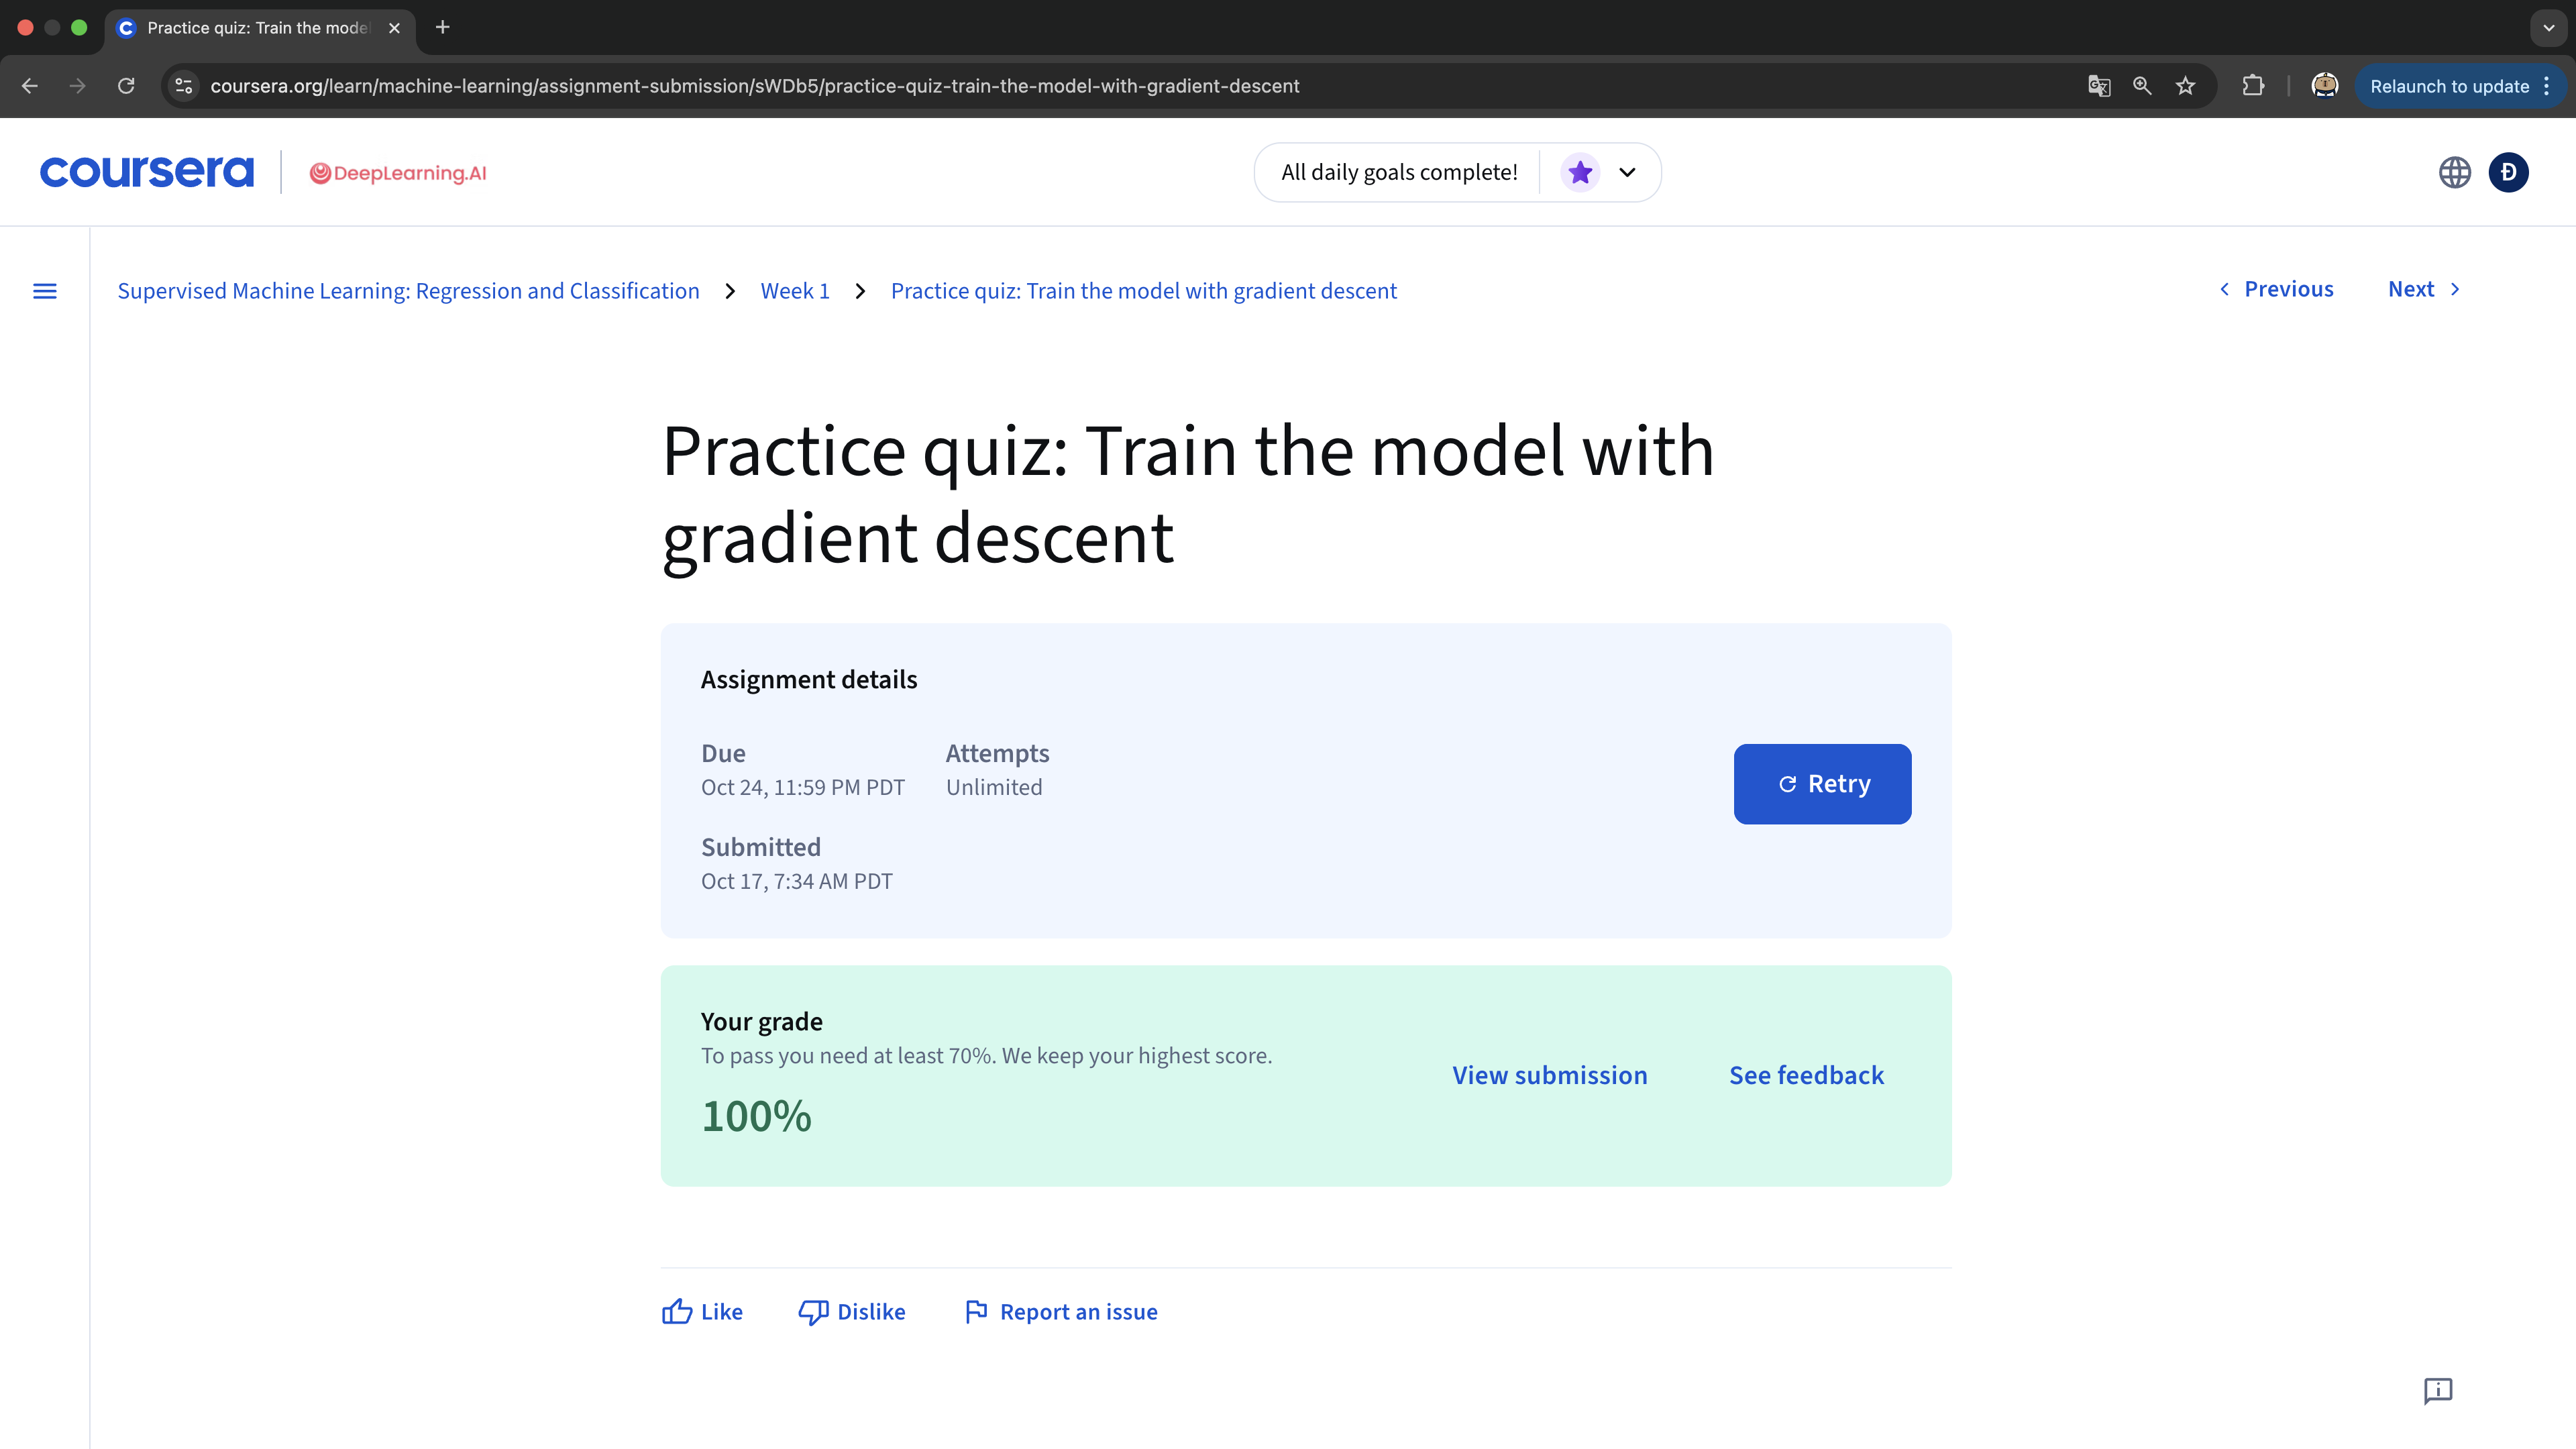
\includegraphics[scale=0.25]{Image/c1_w1_q3.png}
    \caption{Completed Graded Assignment 3 (Train the model with gradient descent)}
\end{figure}

%----------------------------------------
\subsection{Week 2: Regression with Multiple Input Variables}
%----------------------------------------

\subsubsection{Key Insights and Learnings}

This module expanded linear regression to handle complex, real-world datasets with multiple features, focusing on computational efficiency and convergence speed.

\begin{itemize}
    \item \textbf{Vectorization (NumPy):} Leveraged linear algebra principles to process large datasets. By replacing explicit \texttt{for} loops with vector/matrix operations ($np.dot$), computation time is drastically reduced, enabling the training of scalable models.

    \item \textbf{Feature Scaling \& Convergence:}
    \begin{itemize}
        \item \textbf{Problem:} When features have vastly different scales (e.g., price vs. number of bedrooms), the cost function contours become elongated (elliptical), causing Gradient Descent to oscillate and converge slowly.
        \item \textbf{Solution:} Applied \textbf{Z-score Normalization} to rescale features. This transforms the cost function contours into circles, allowing Gradient Descent to take a direct path to the minimum.
    \end{itemize}

    \item \textbf{Feature Engineering and Polynomial Regression:} Learned that model power isn't limited by linear features. By engineering new features (e.g., $x^2, x^3, \sqrt{x}$), a linear model can be adapted to fit non-linear curves, enhancing flexibility without changing the underlying optimization algorithm.
\end{itemize}

\subsubsection{Learning Evidence}
\begin{figure}[H]
    \centering
    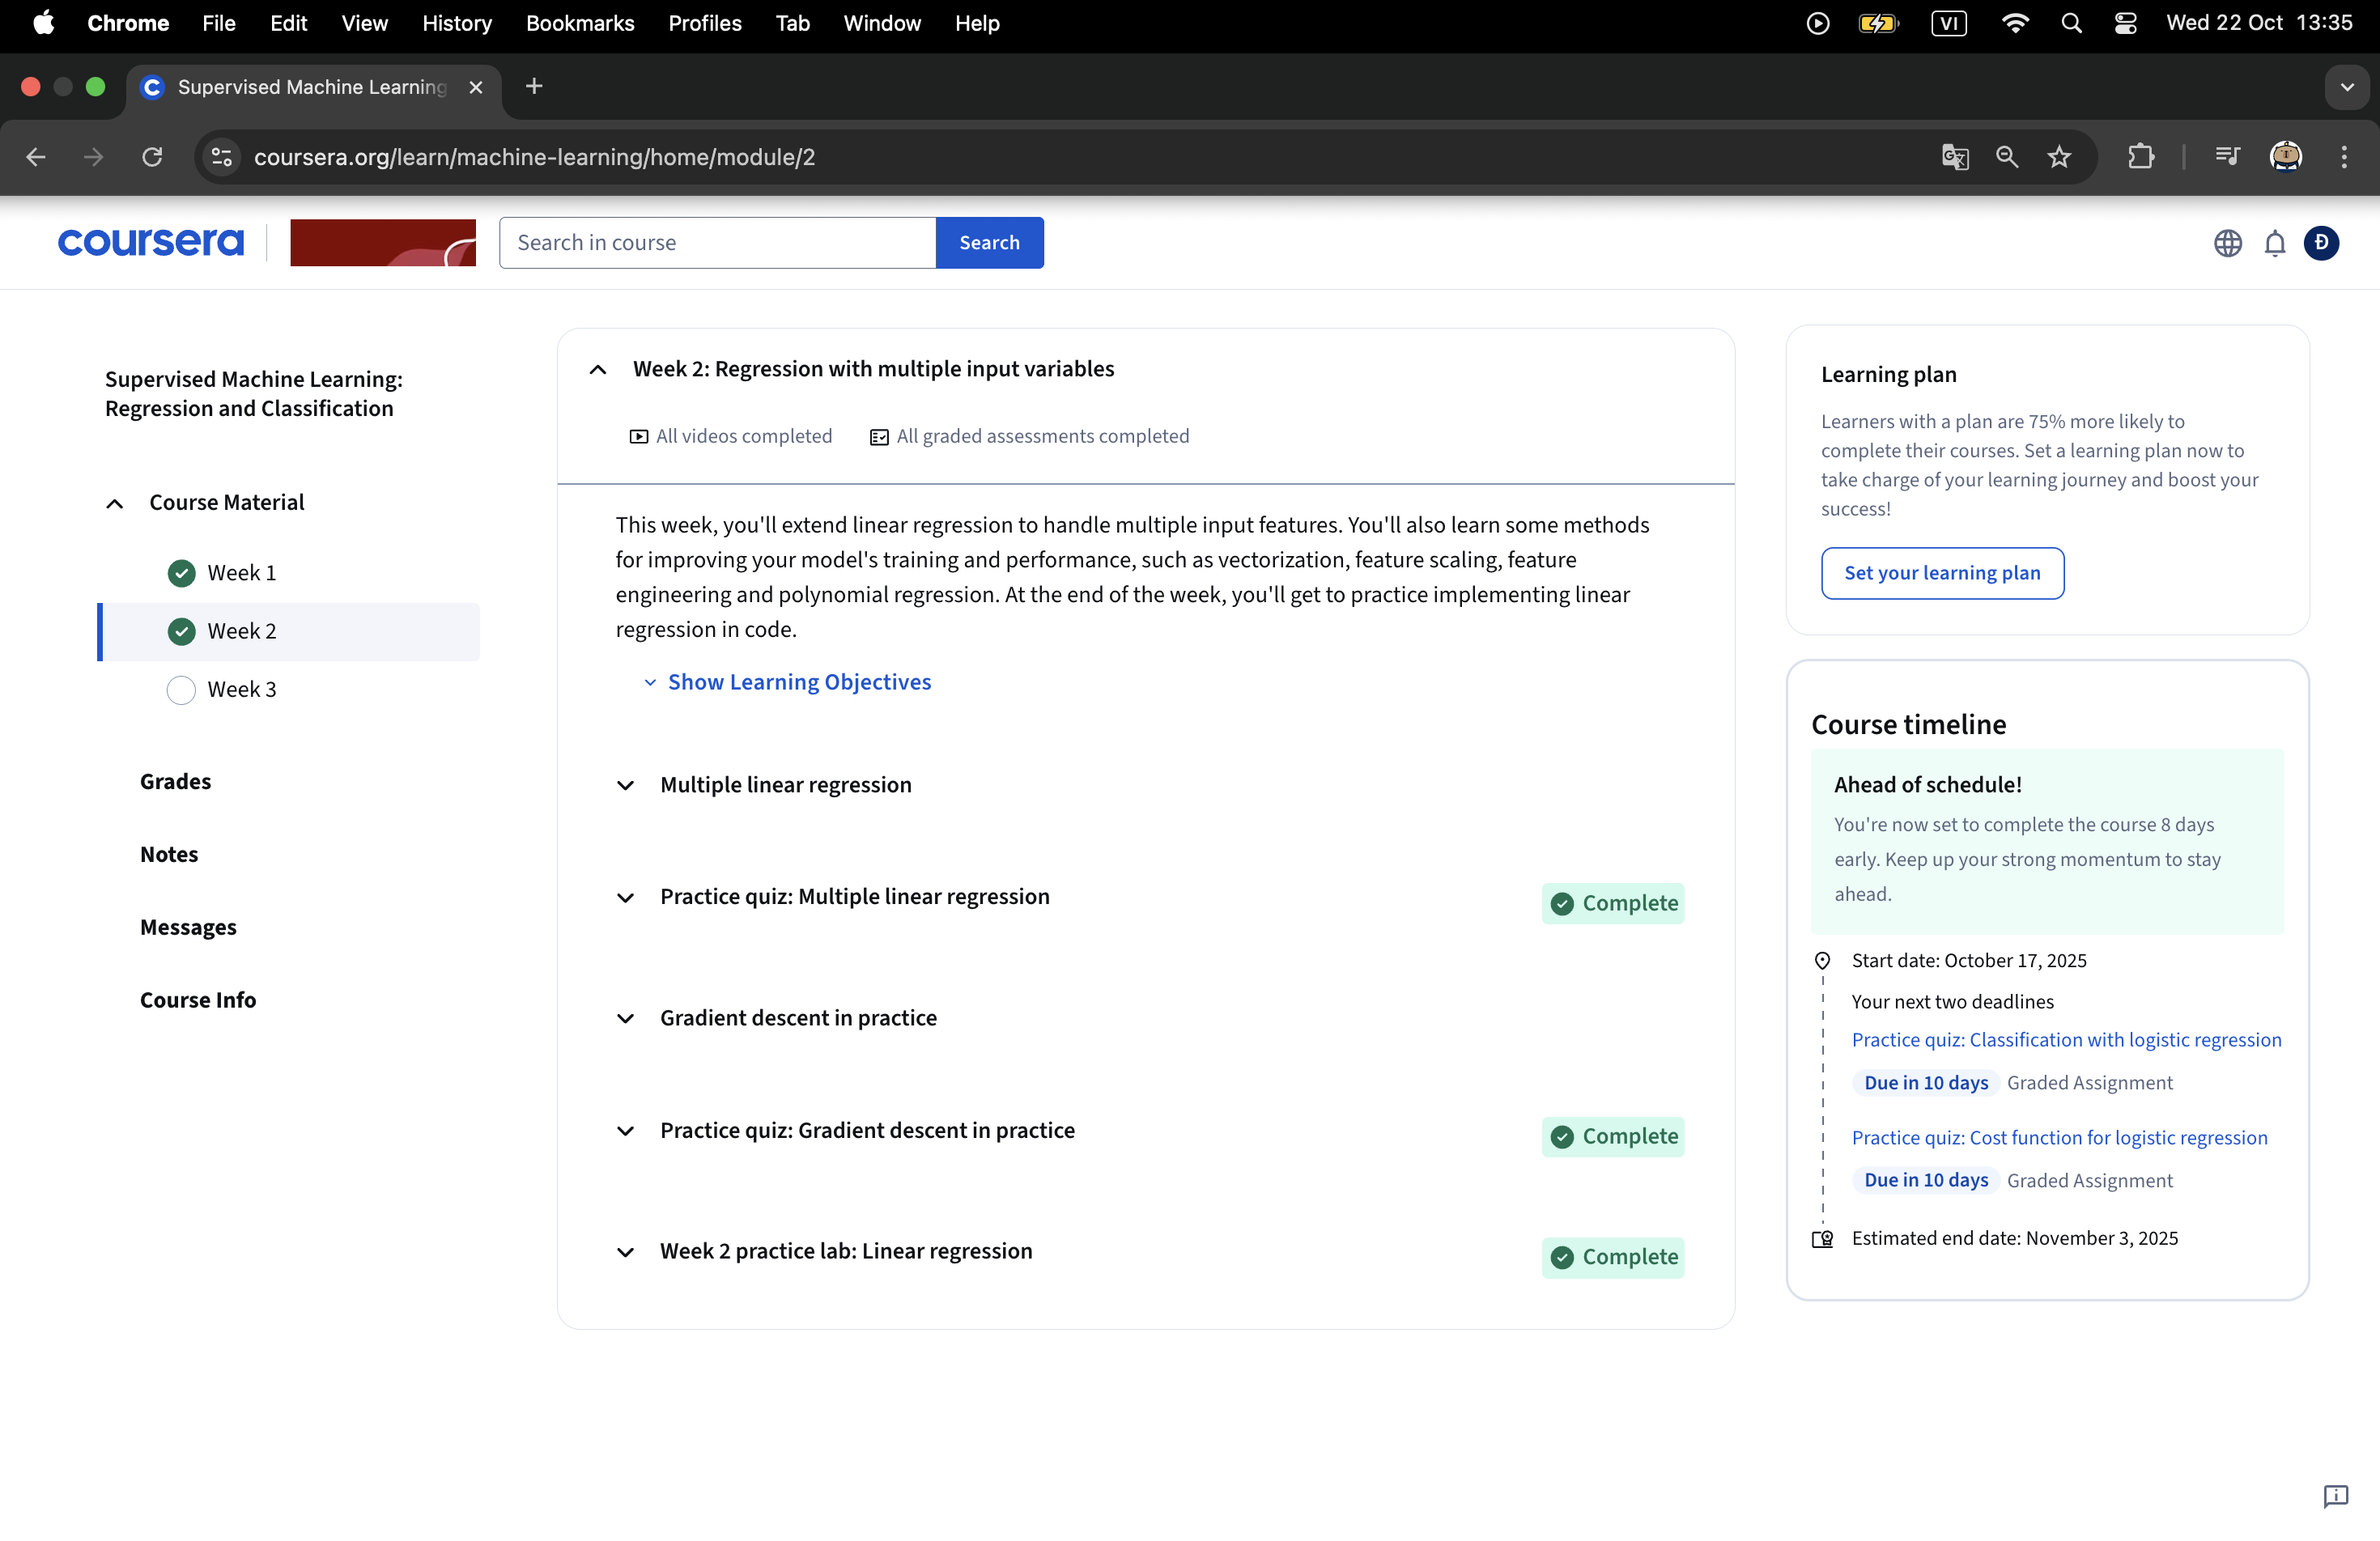
\includegraphics[scale=0.25]{Image/c1_w2.png}
    \caption{Lesson's completed date (22/10/2025)}
\end{figure}

\subsubsection{Graded Assignment Evidence}
\begin{figure}[H]
    \centering
    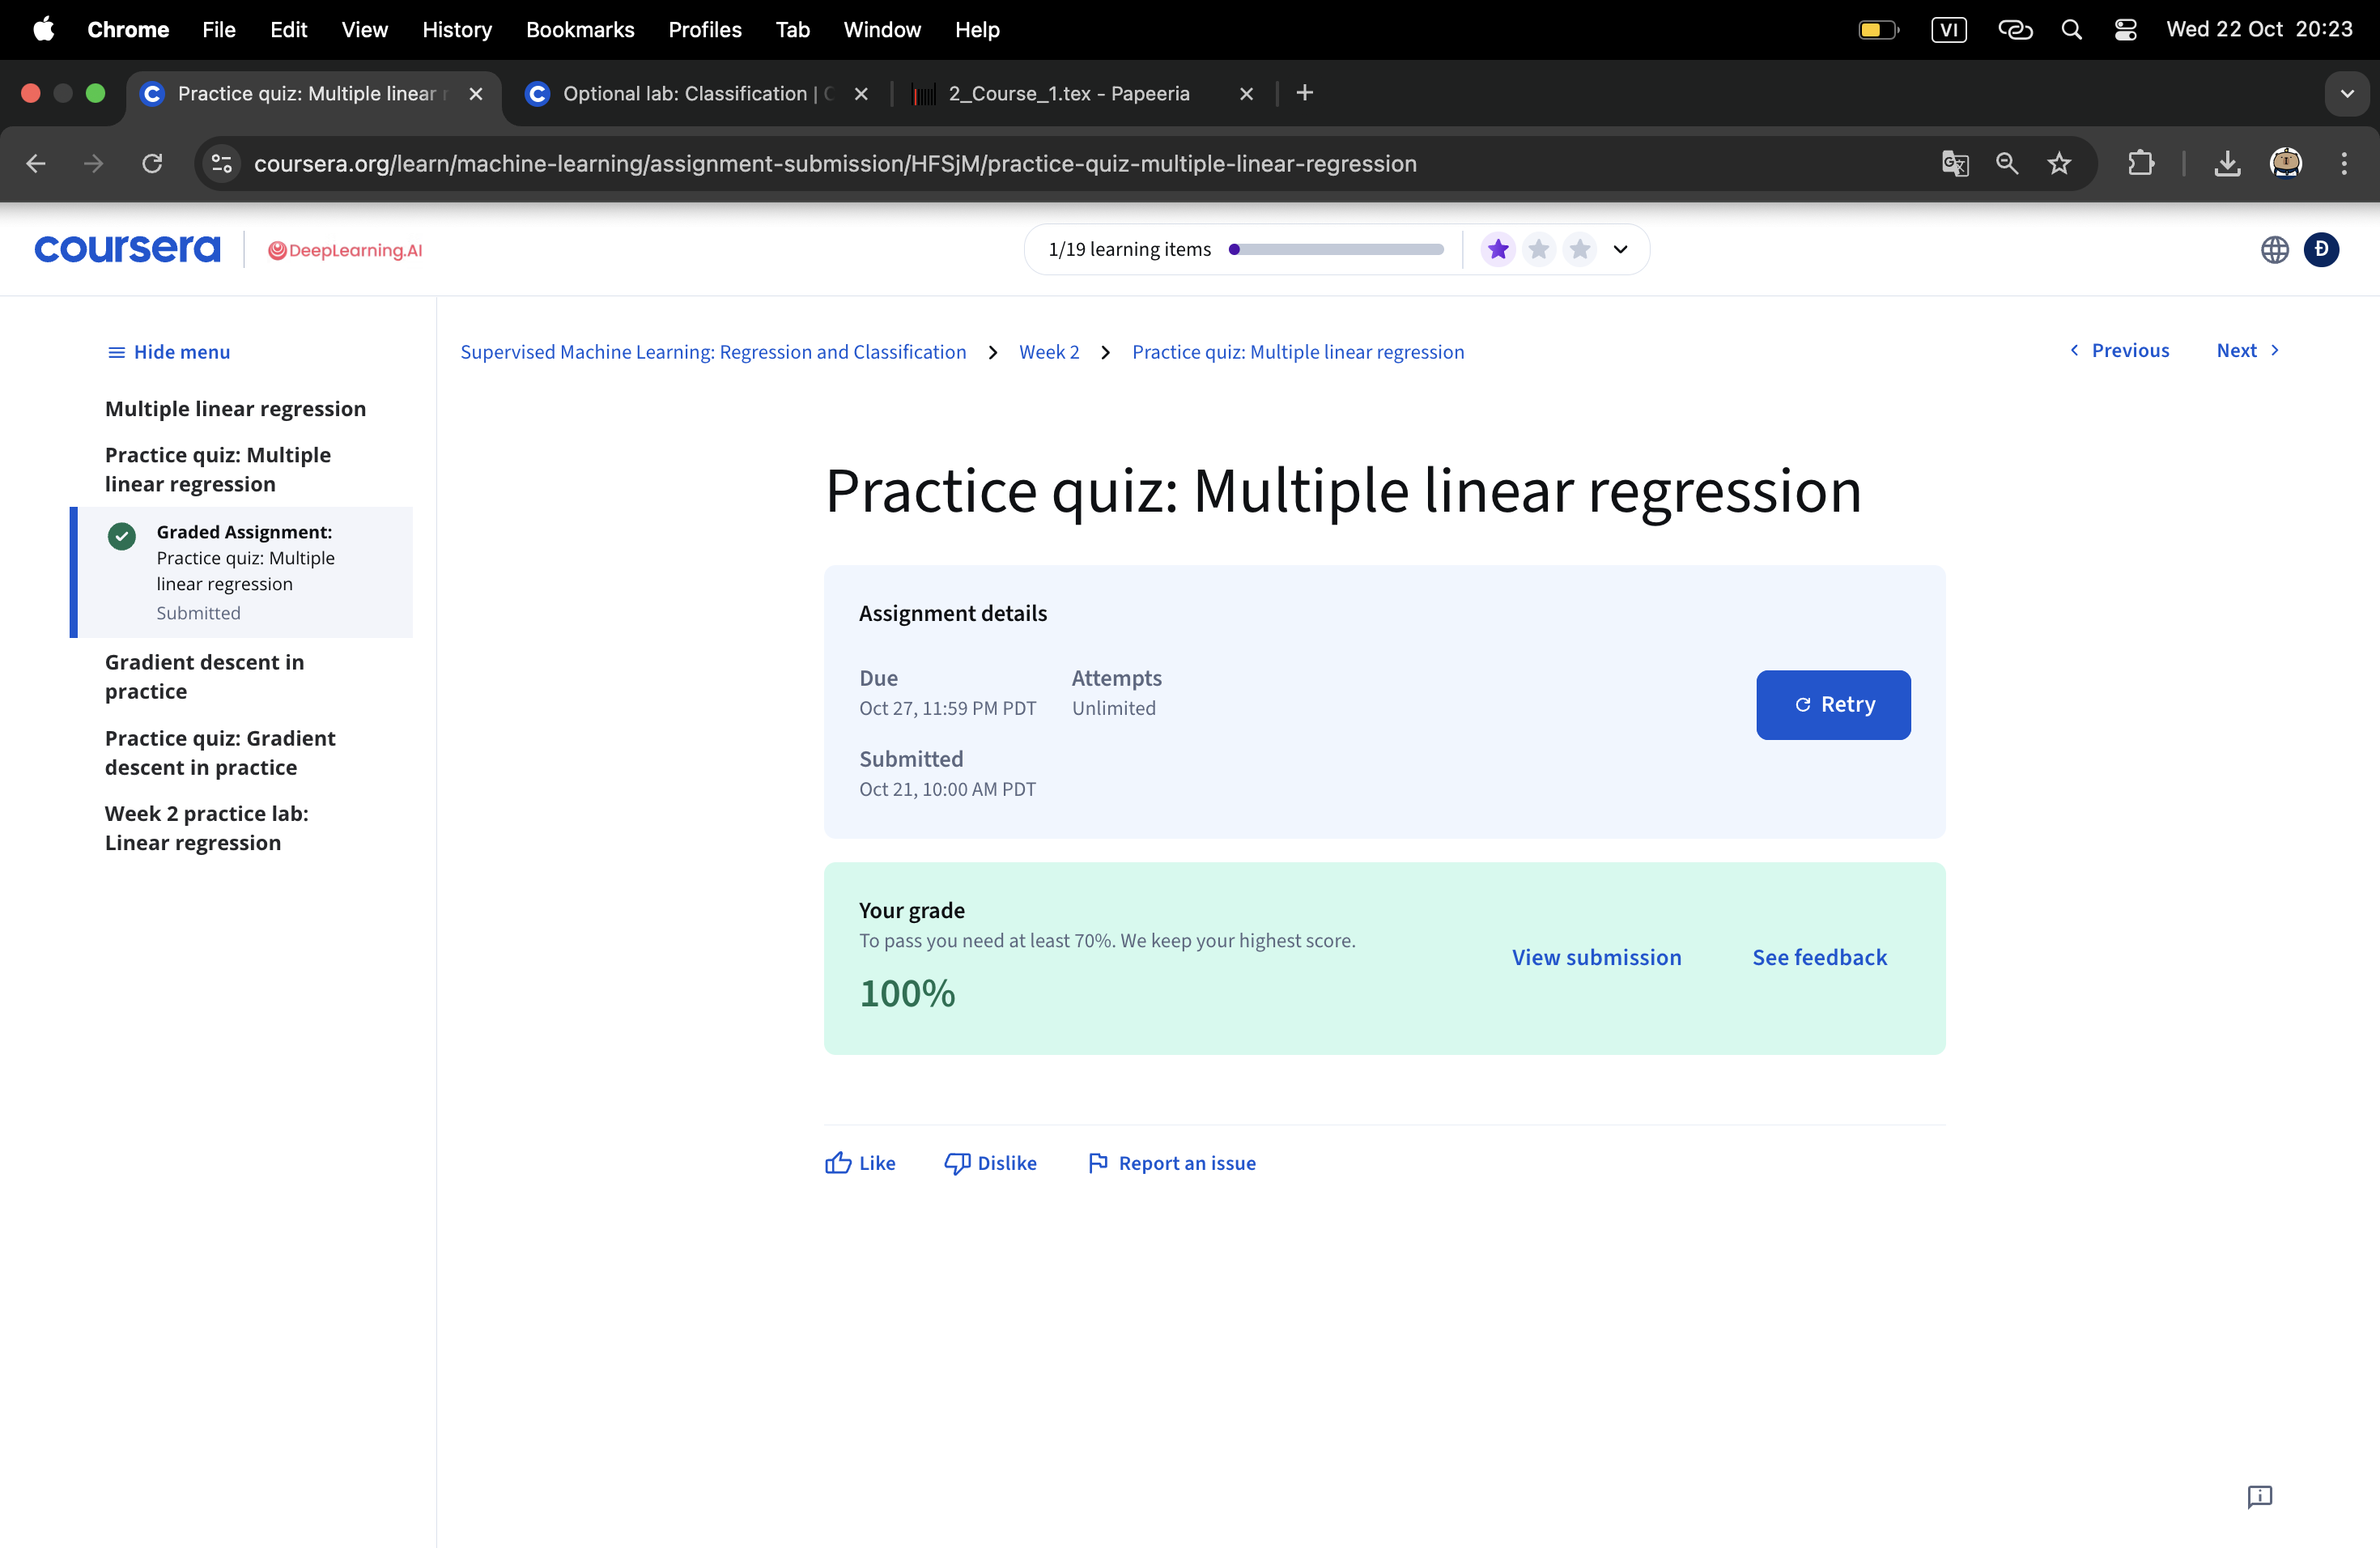
\includegraphics[scale=0.25]{Image/c1_w2_q1.png}
    \caption{Completed Graded Assignment 1 (Multiple linear regression)}
\end{figure}

\begin{figure}[H]
    \centering
    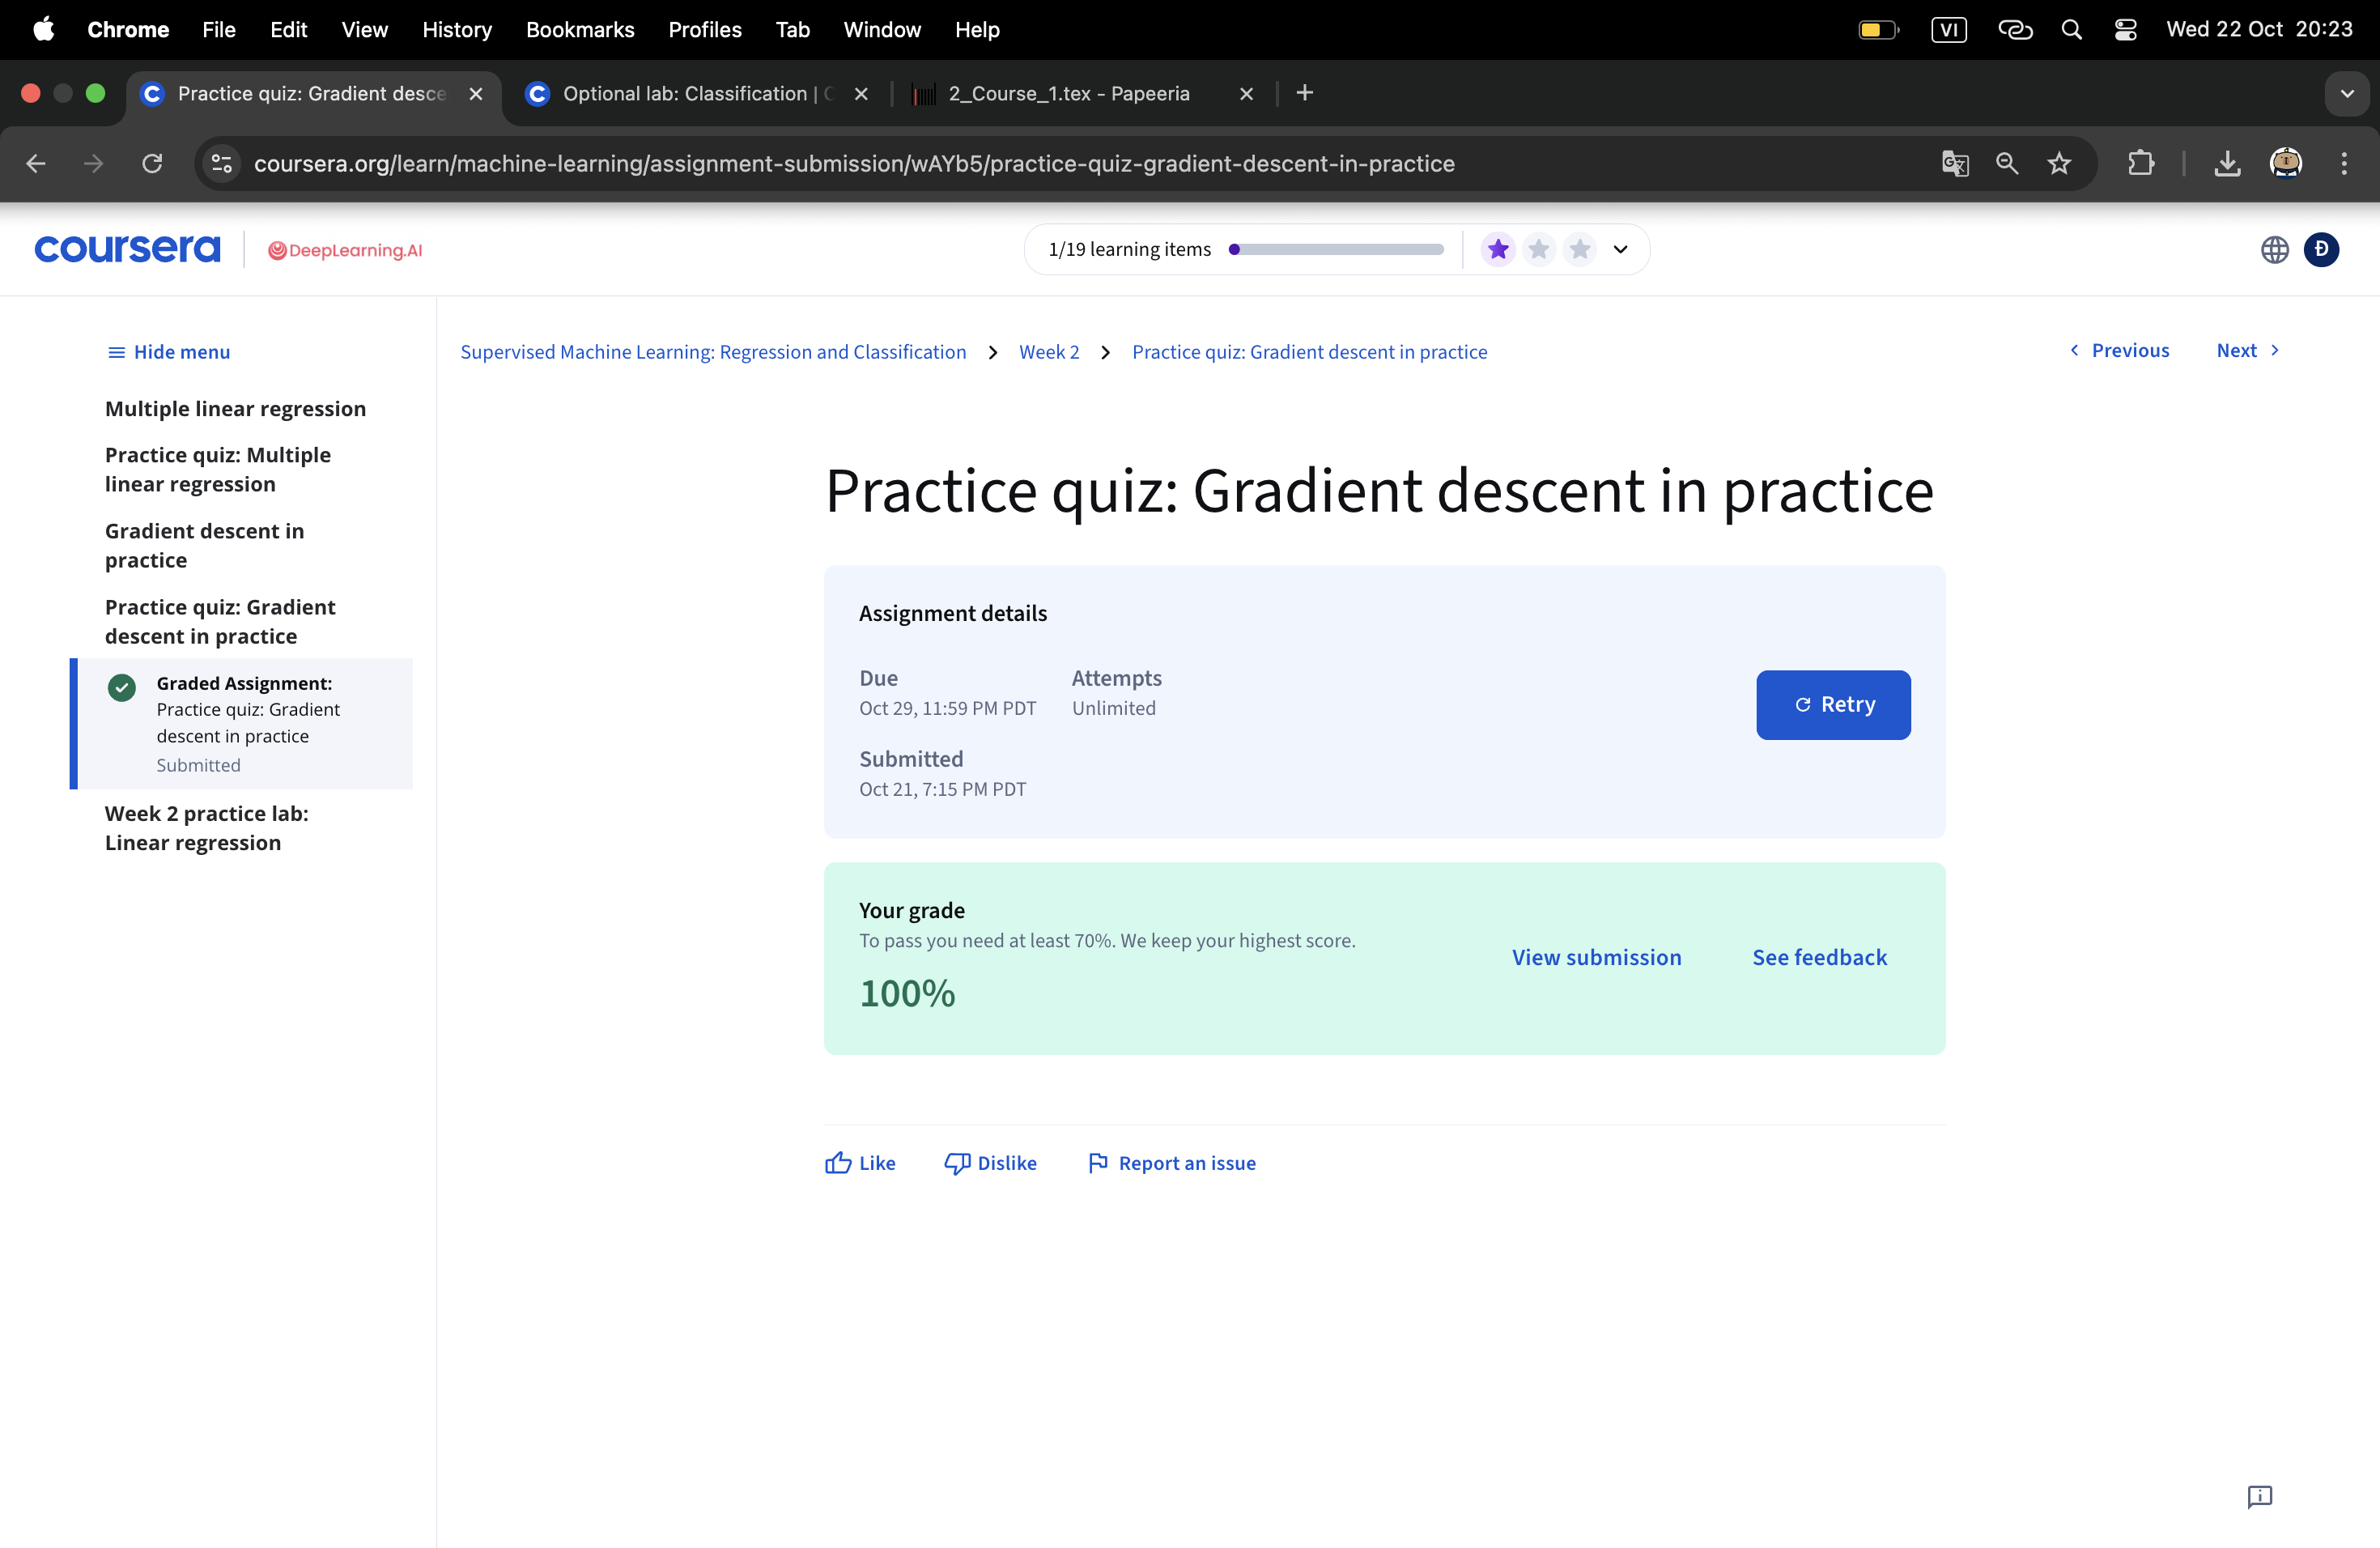
\includegraphics[scale=0.25]{Image/c1_w2_q2.png}
    \caption{Completed Graded Assignment 2 (Gradient descent in practice)}
\end{figure}

\begin{figure}[H]
    \centering
    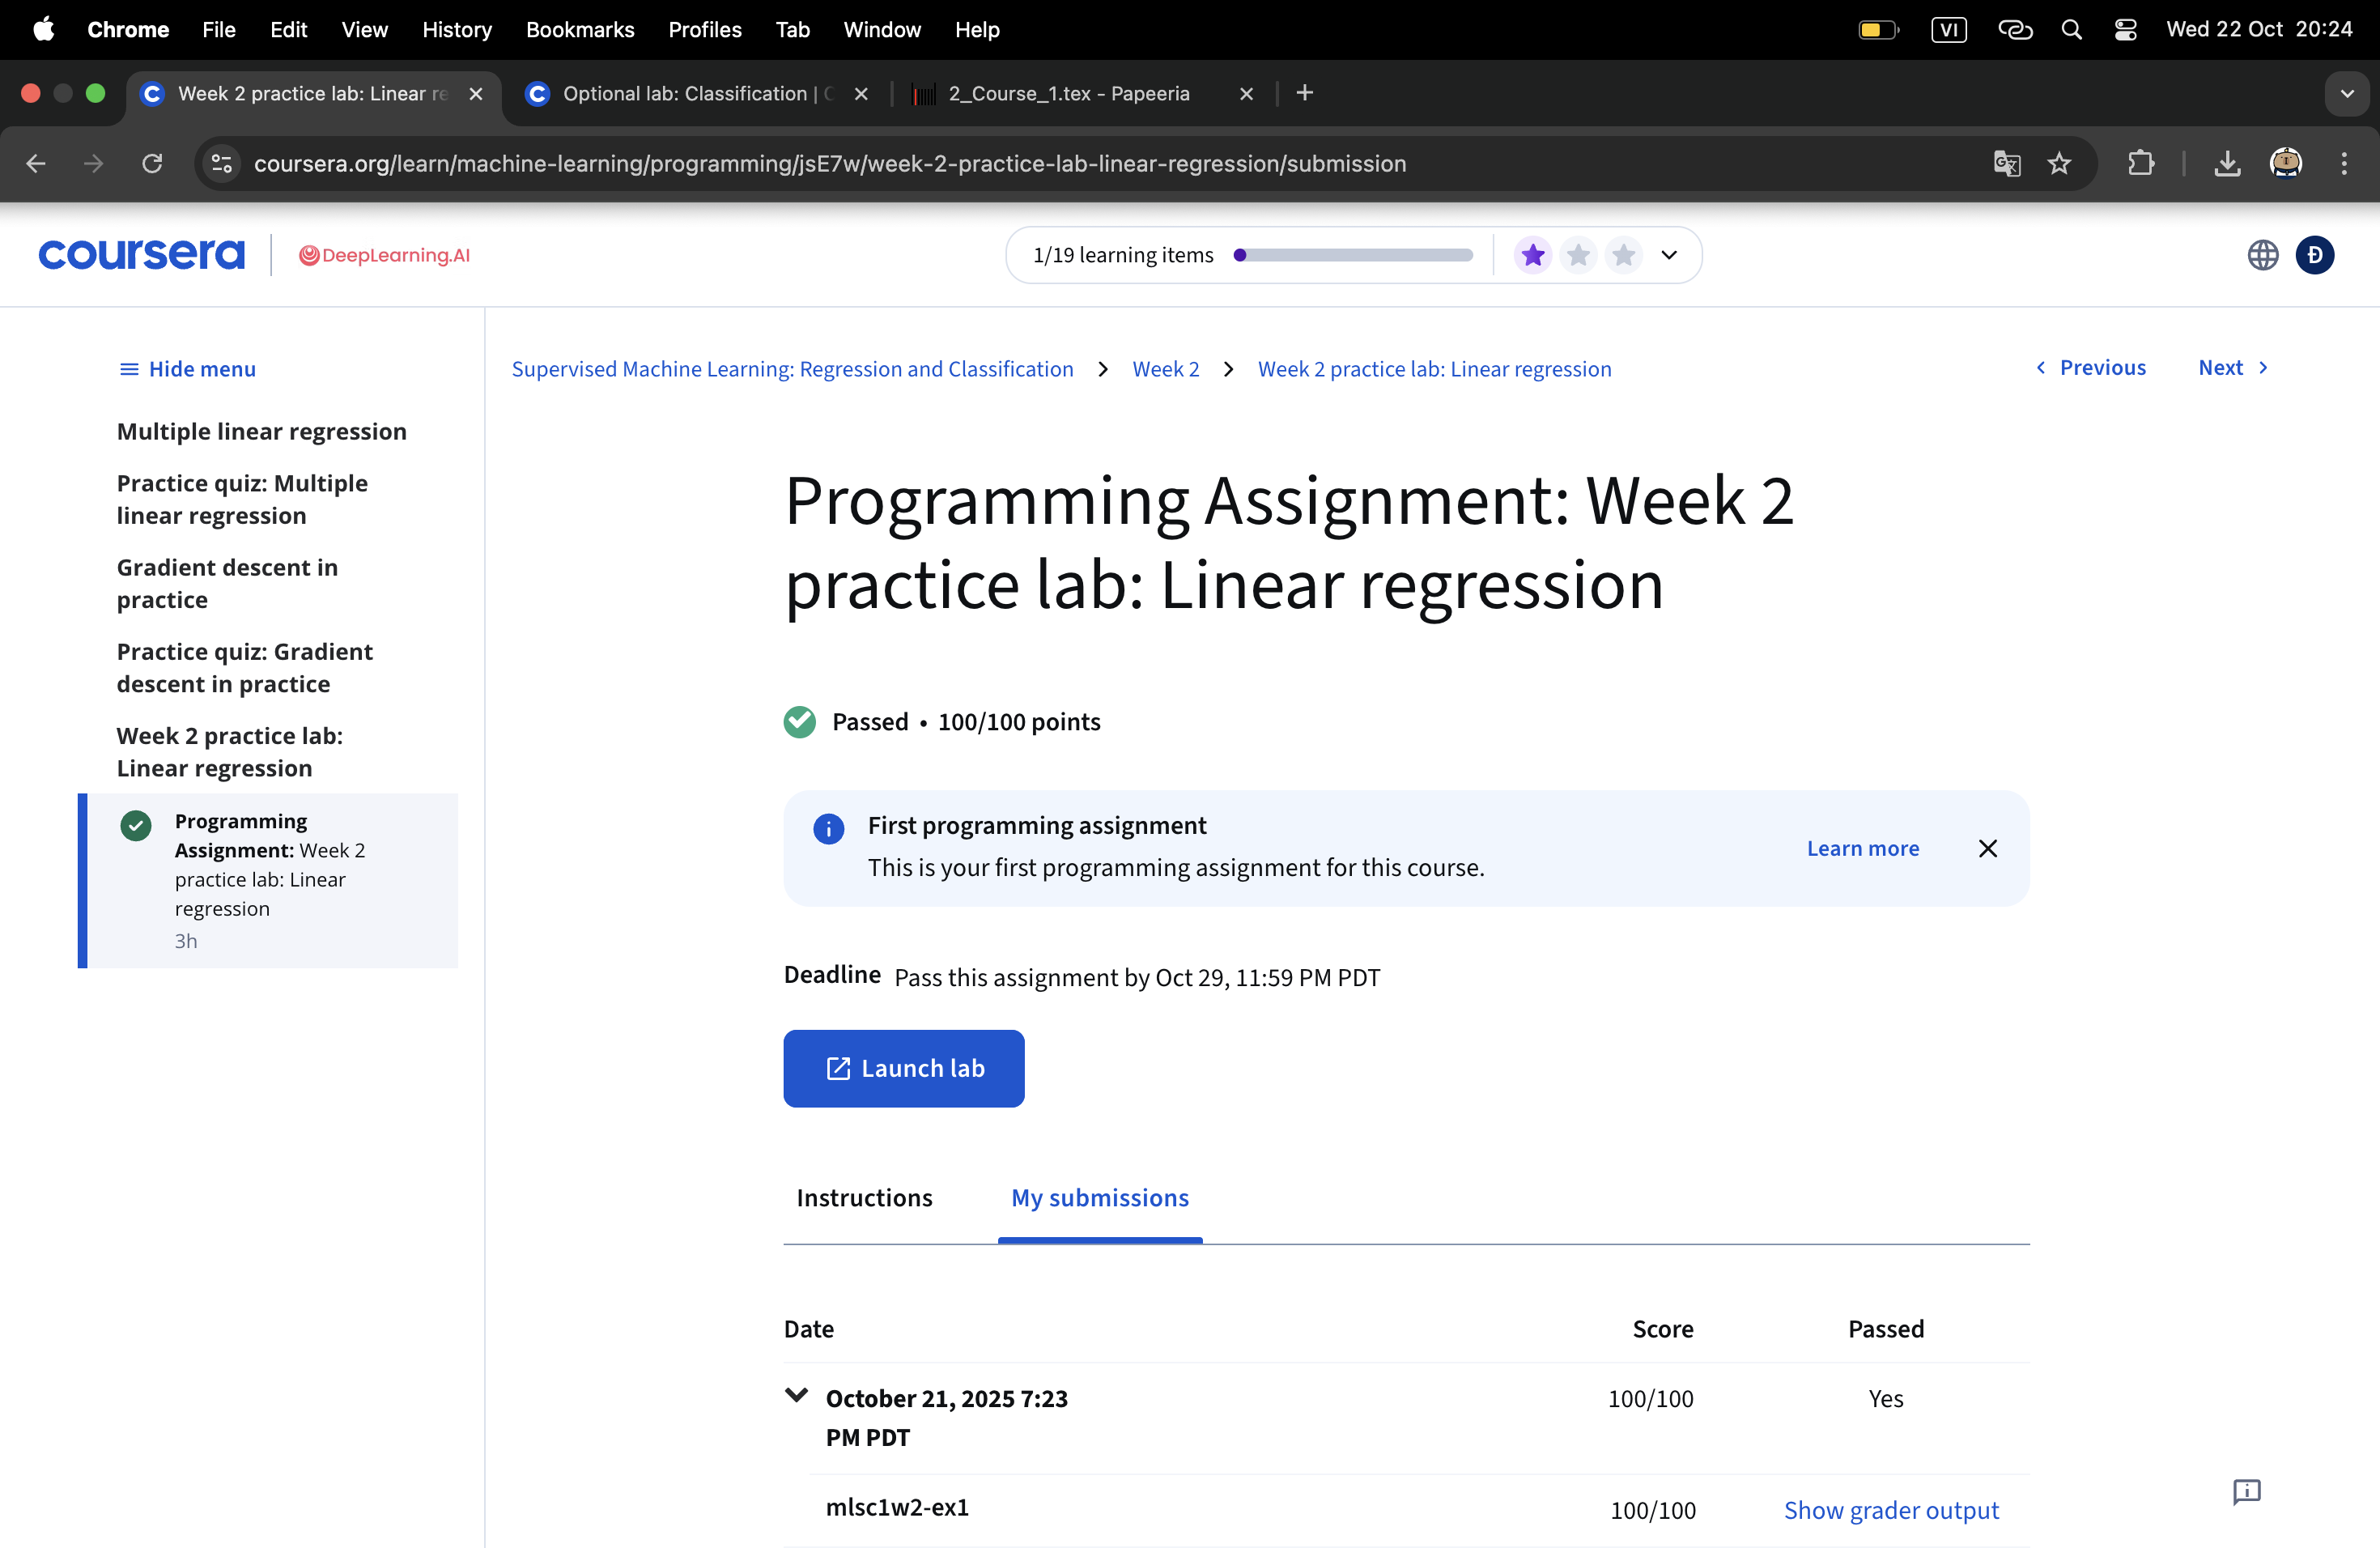
\includegraphics[scale=0.25]{Image/c1_w2_q3.png}
    \caption{Completed Programming Assignment (Linear regression)}
\end{figure}

%----------------------------------------
\subsection{Week 3: Classification}
%----------------------------------------

\subsubsection{Key Insights and Learnings}

This module introduced the mathematical adaptations required to predict categories rather than continuous numbers.

\begin{itemize}
    \item \textbf{Logistic Regression and The Sigmoid Function:} 
    \begin{itemize}
        \item Addressed the limitations of linear regression for classification (unbounded output).
        \item Applied the \textbf{Sigmoid Function} ($g(z) = \frac{1}{1+e^{-z}}$) to map predictions to a probability range $[0, 1]$, interpreting the output as $P(y=1|x)$.
    \end{itemize}

    \item \textbf{Decision Boundaries:} Visualized classification not just as a prediction task, but as finding a geometric boundary (line or polynomial curve) that separates different classes in the feature space.

    \item \textbf{The Logistic Loss Function:} 
    \begin{itemize}
        \item Learned that using MSE for Logistic Regression results in a \textbf{non-convex} cost function (many local minima).
        \item Implemented the \textbf{Log Loss (Binary Cross-Entropy)} function to ensure the cost function is convex, guaranteeing that Gradient Descent can find the global optimum.
    \end{itemize}

    \item \textbf{Overfitting and Regularization:} 
    \begin{itemize}
        \item \textbf{The Problem:} Models that fit training data too closely (high variance) fail to generalize to new data.
        \item \textbf{The Solution:} Implemented \textbf{L2 Regularization}. By adding a penalty term ($\lambda \sum w_j^2$) to the cost function, the model is forced to keep weights small, resulting in a simpler, smoother decision boundary that generalizes better.
    \end{itemize}
\end{itemize}

\subsubsection{Learning Evidence}
\begin{figure}[H]
    \centering
    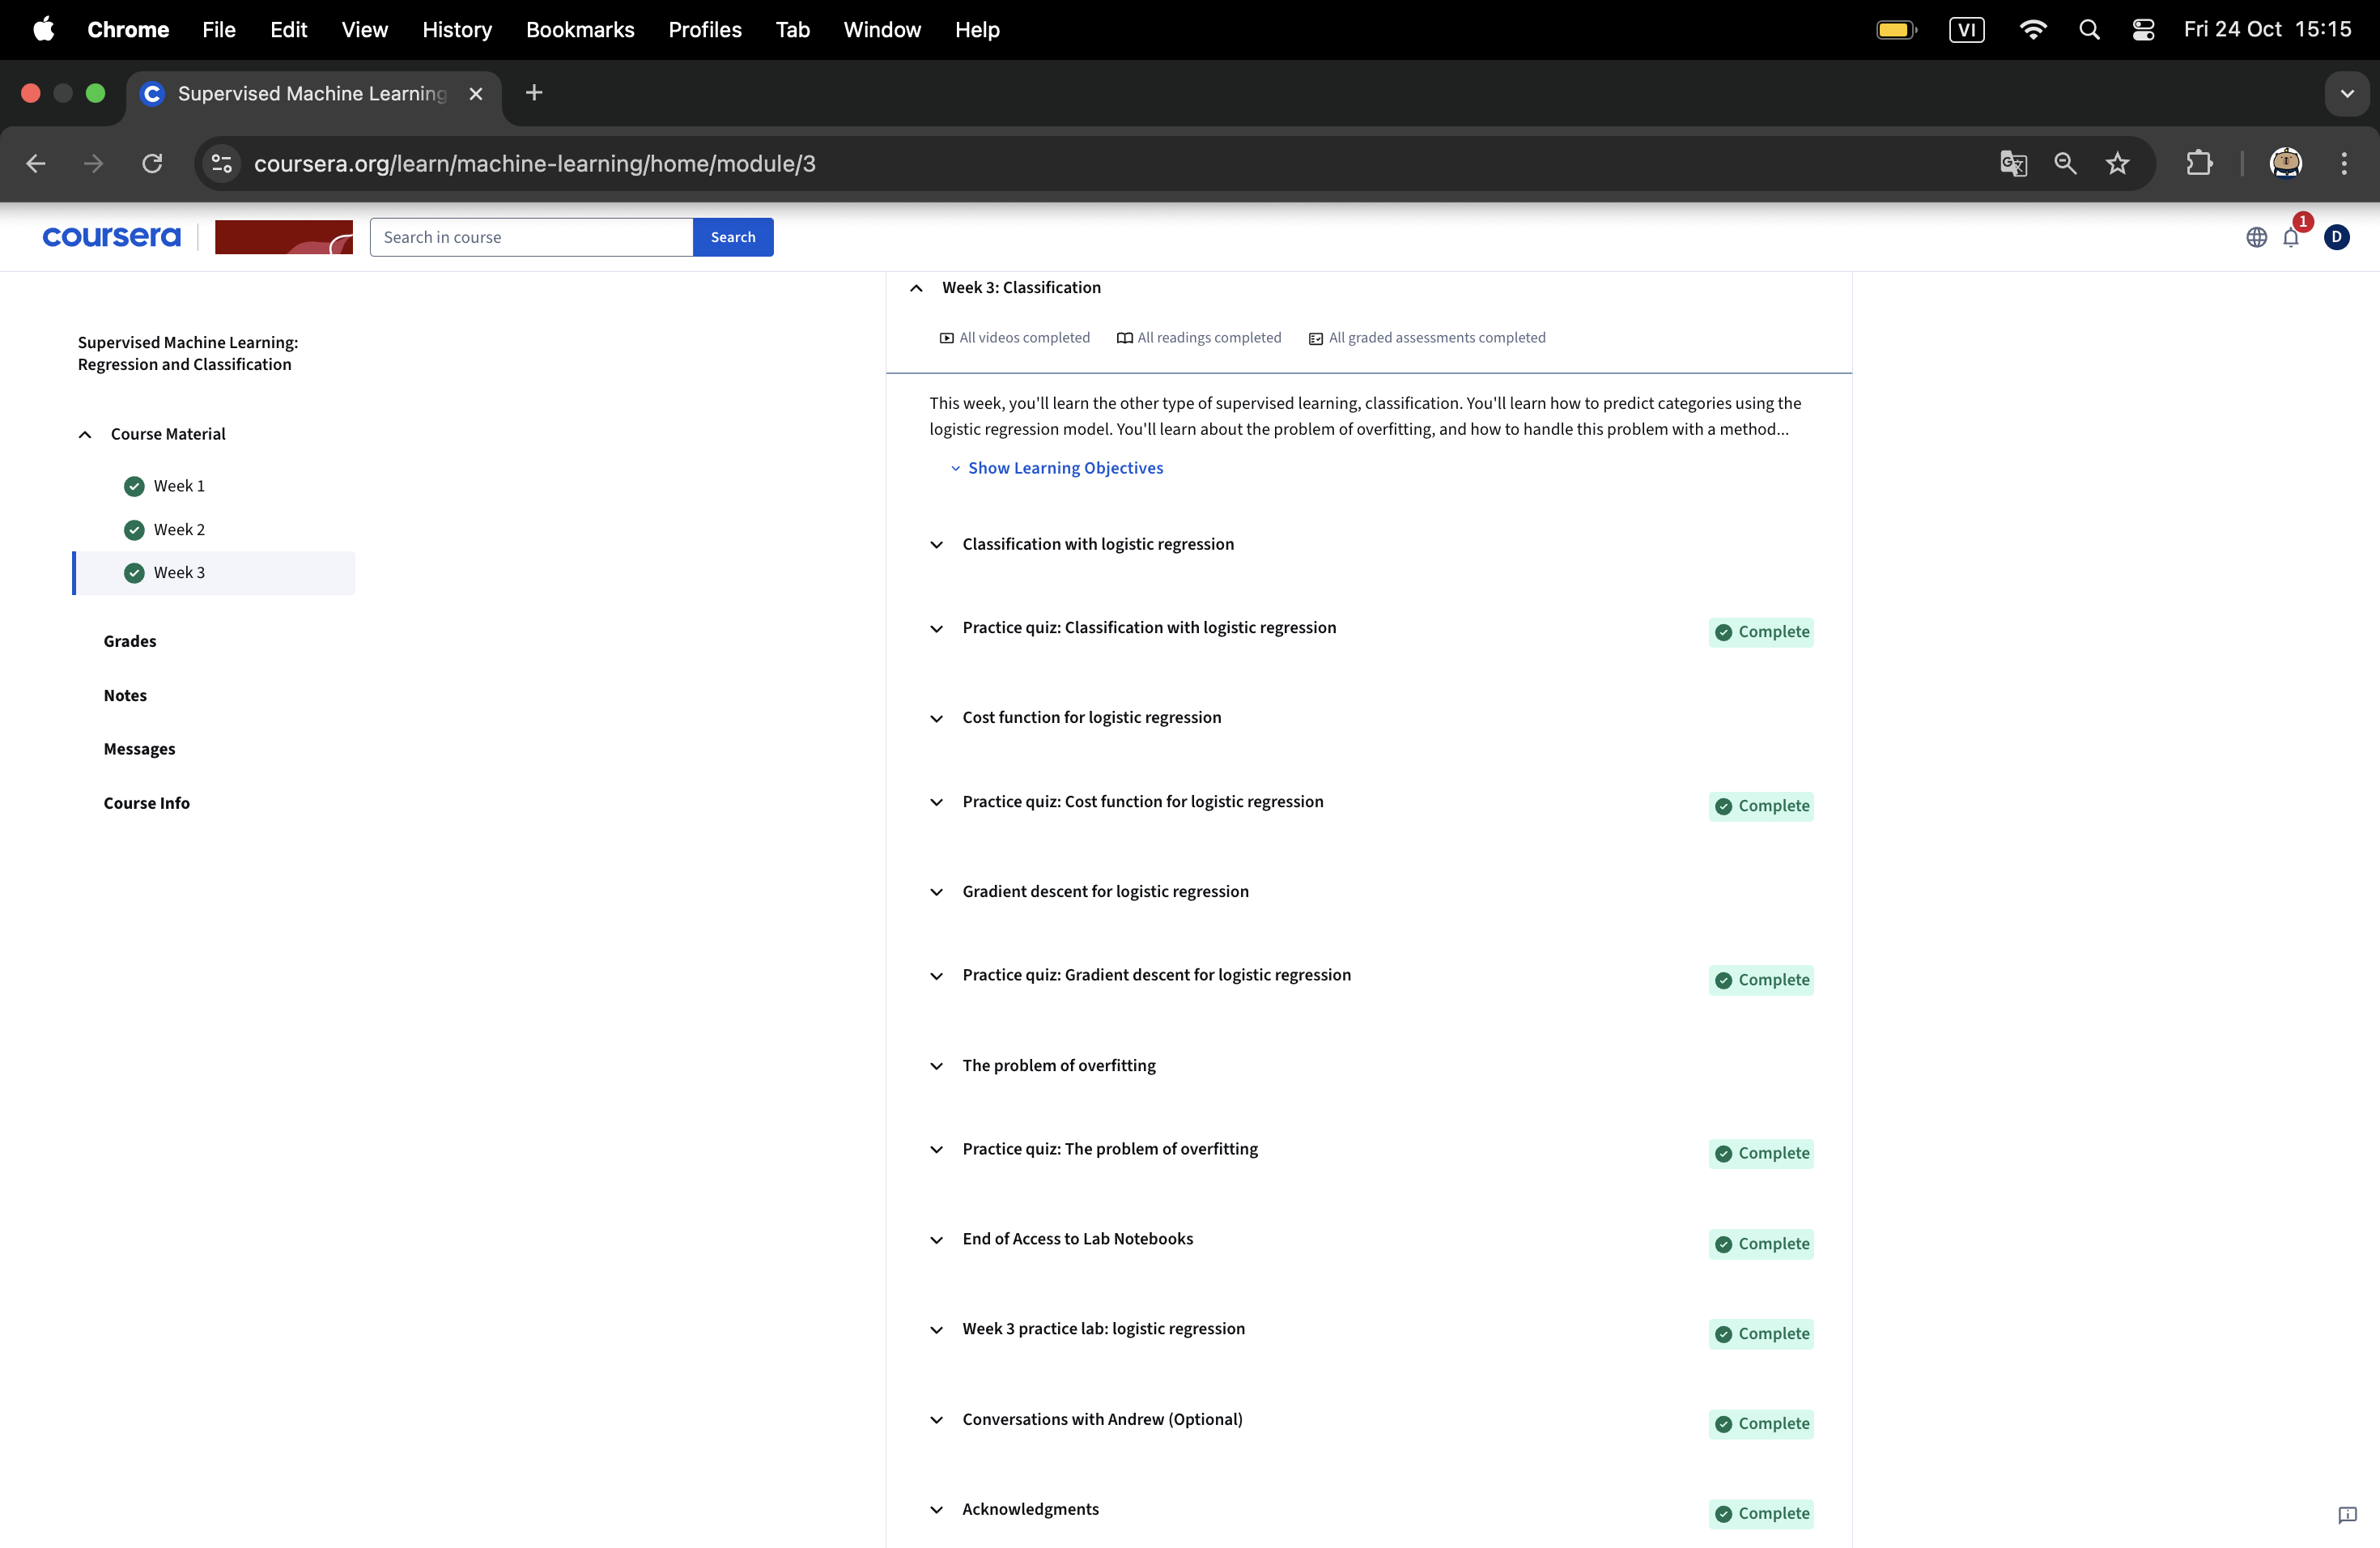
\includegraphics[scale=0.25]{Image/c1_w3.png}
    \caption{Lesson's completed date (24/10/2025)}
\end{figure}

\subsubsection{Graded Assignment Evidence}
\begin{figure}[H]
    \centering
    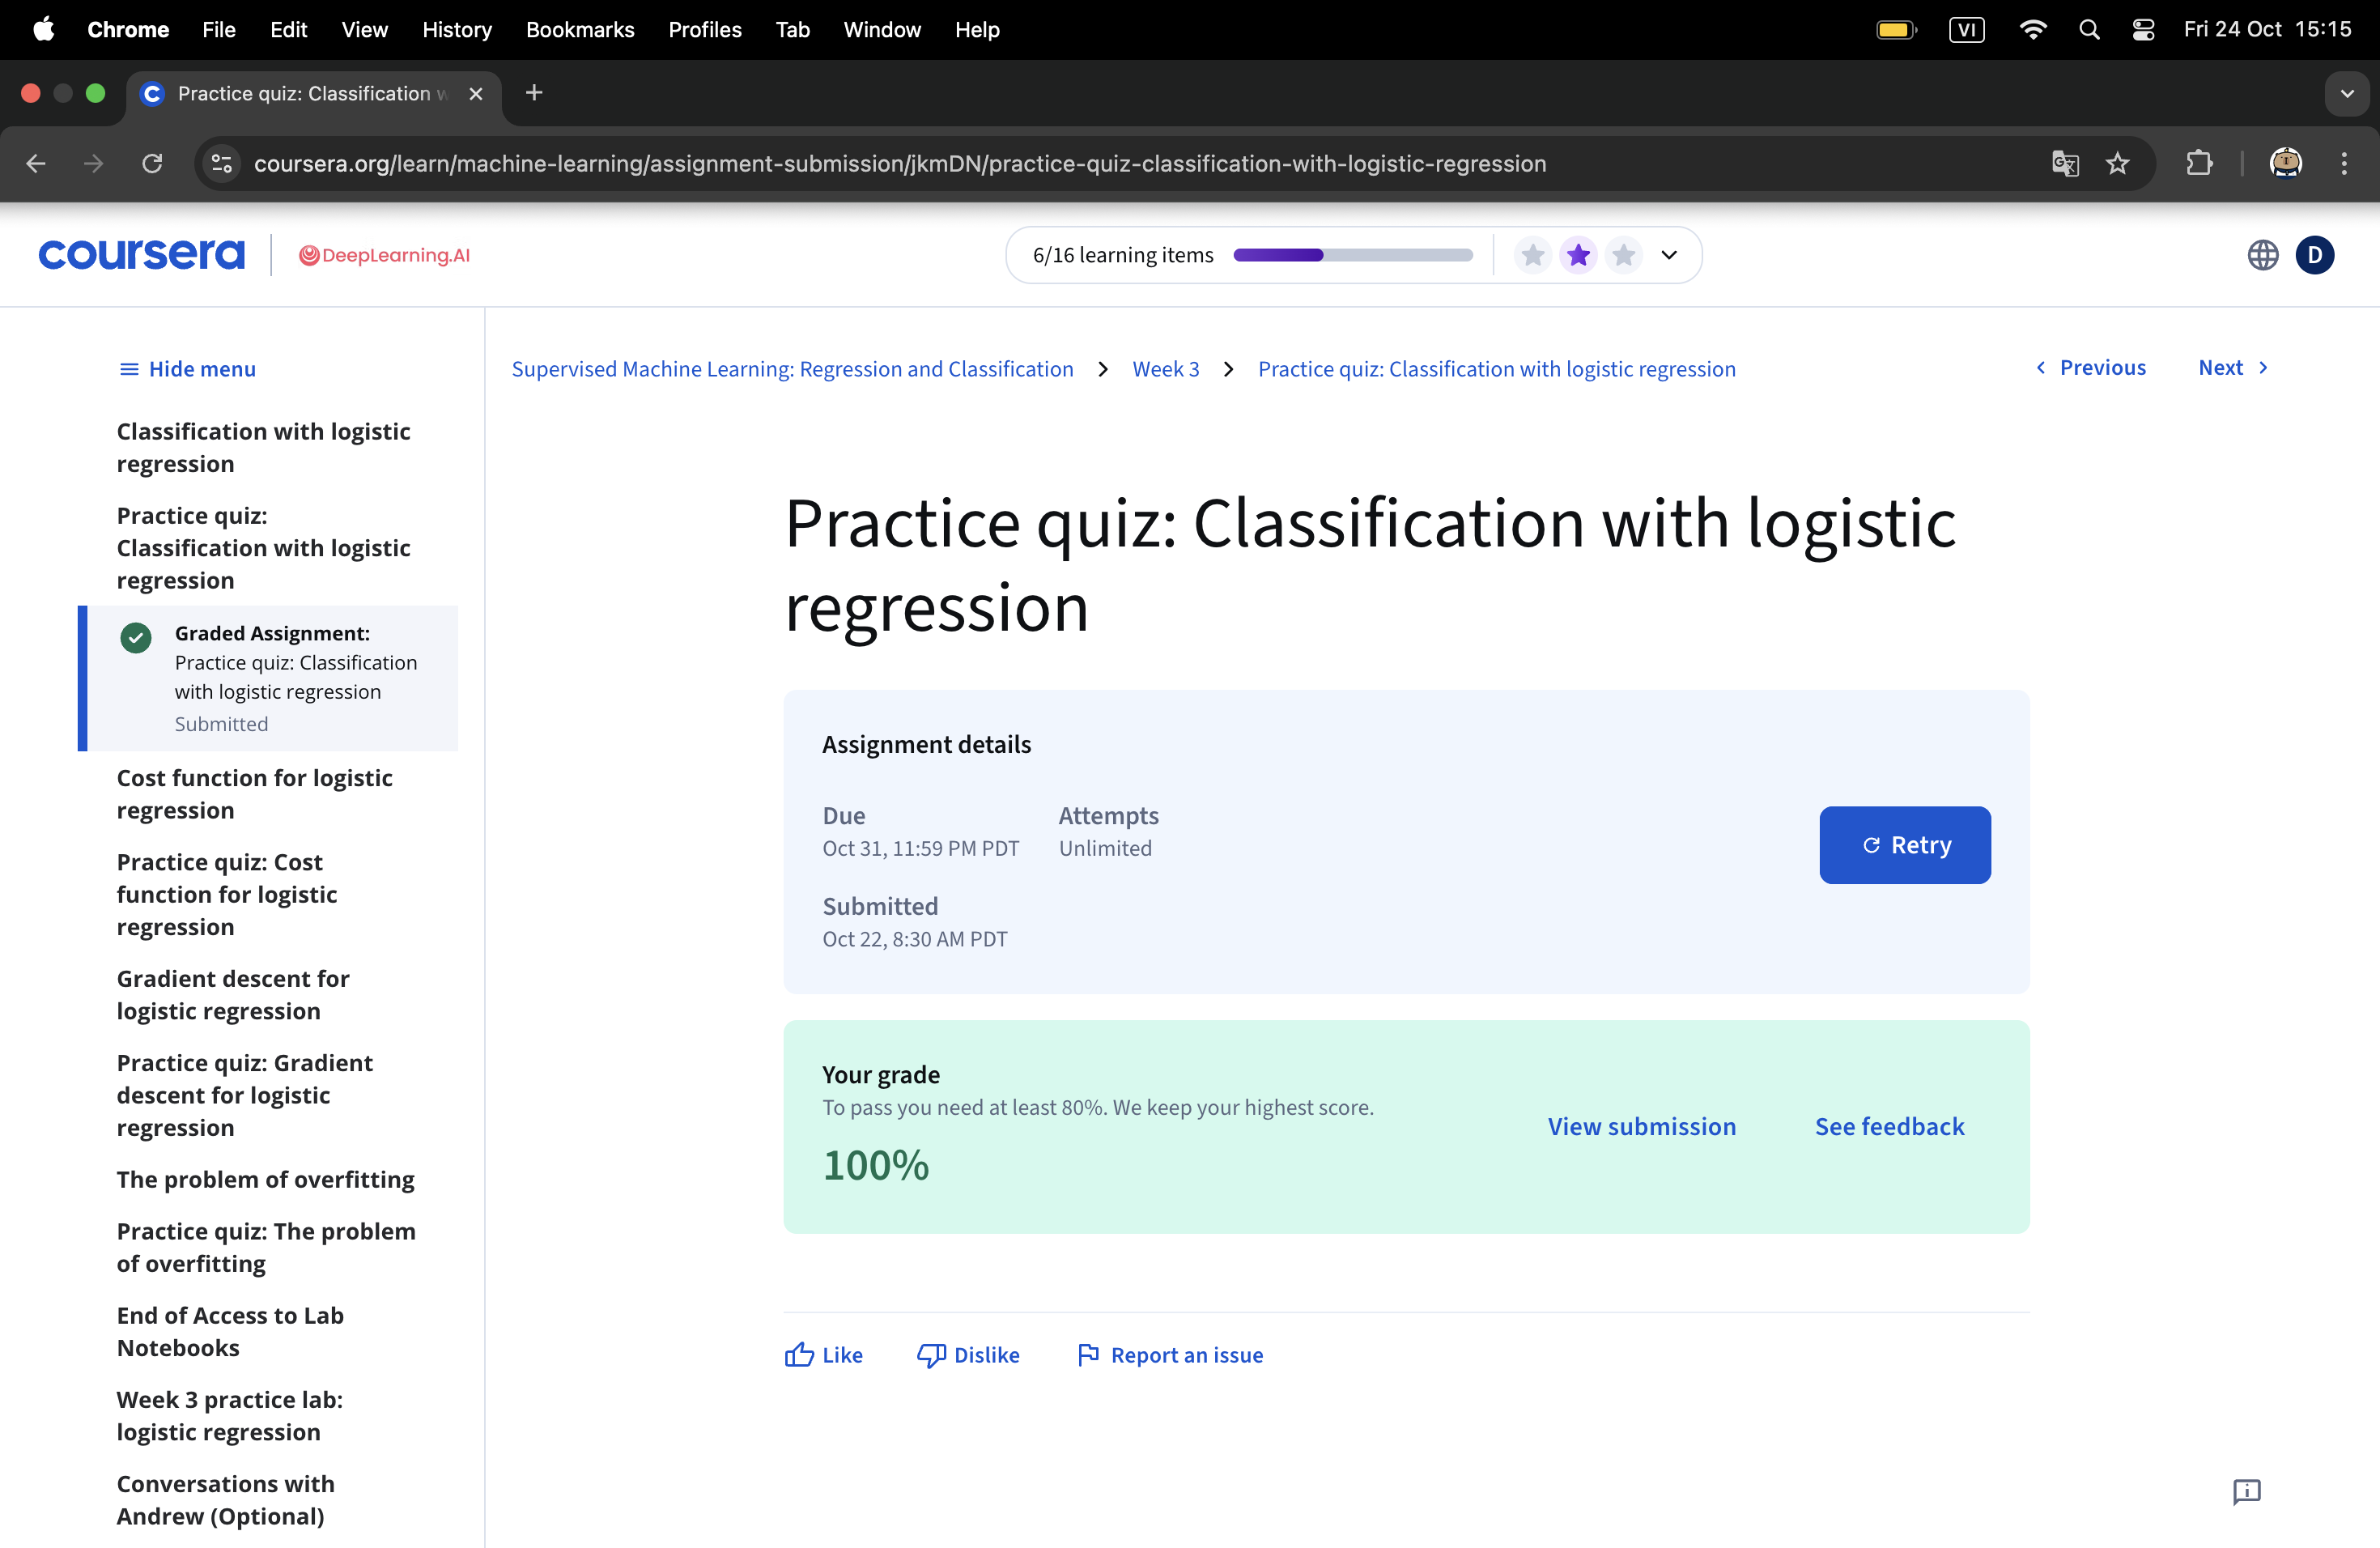
\includegraphics[scale=0.25]{Image/c1_w3_q1.png}
    \caption{Completed Graded Assignment 1 (Classification with logistic regression)}
\end{figure}

\begin{figure}[H]
    \centering
    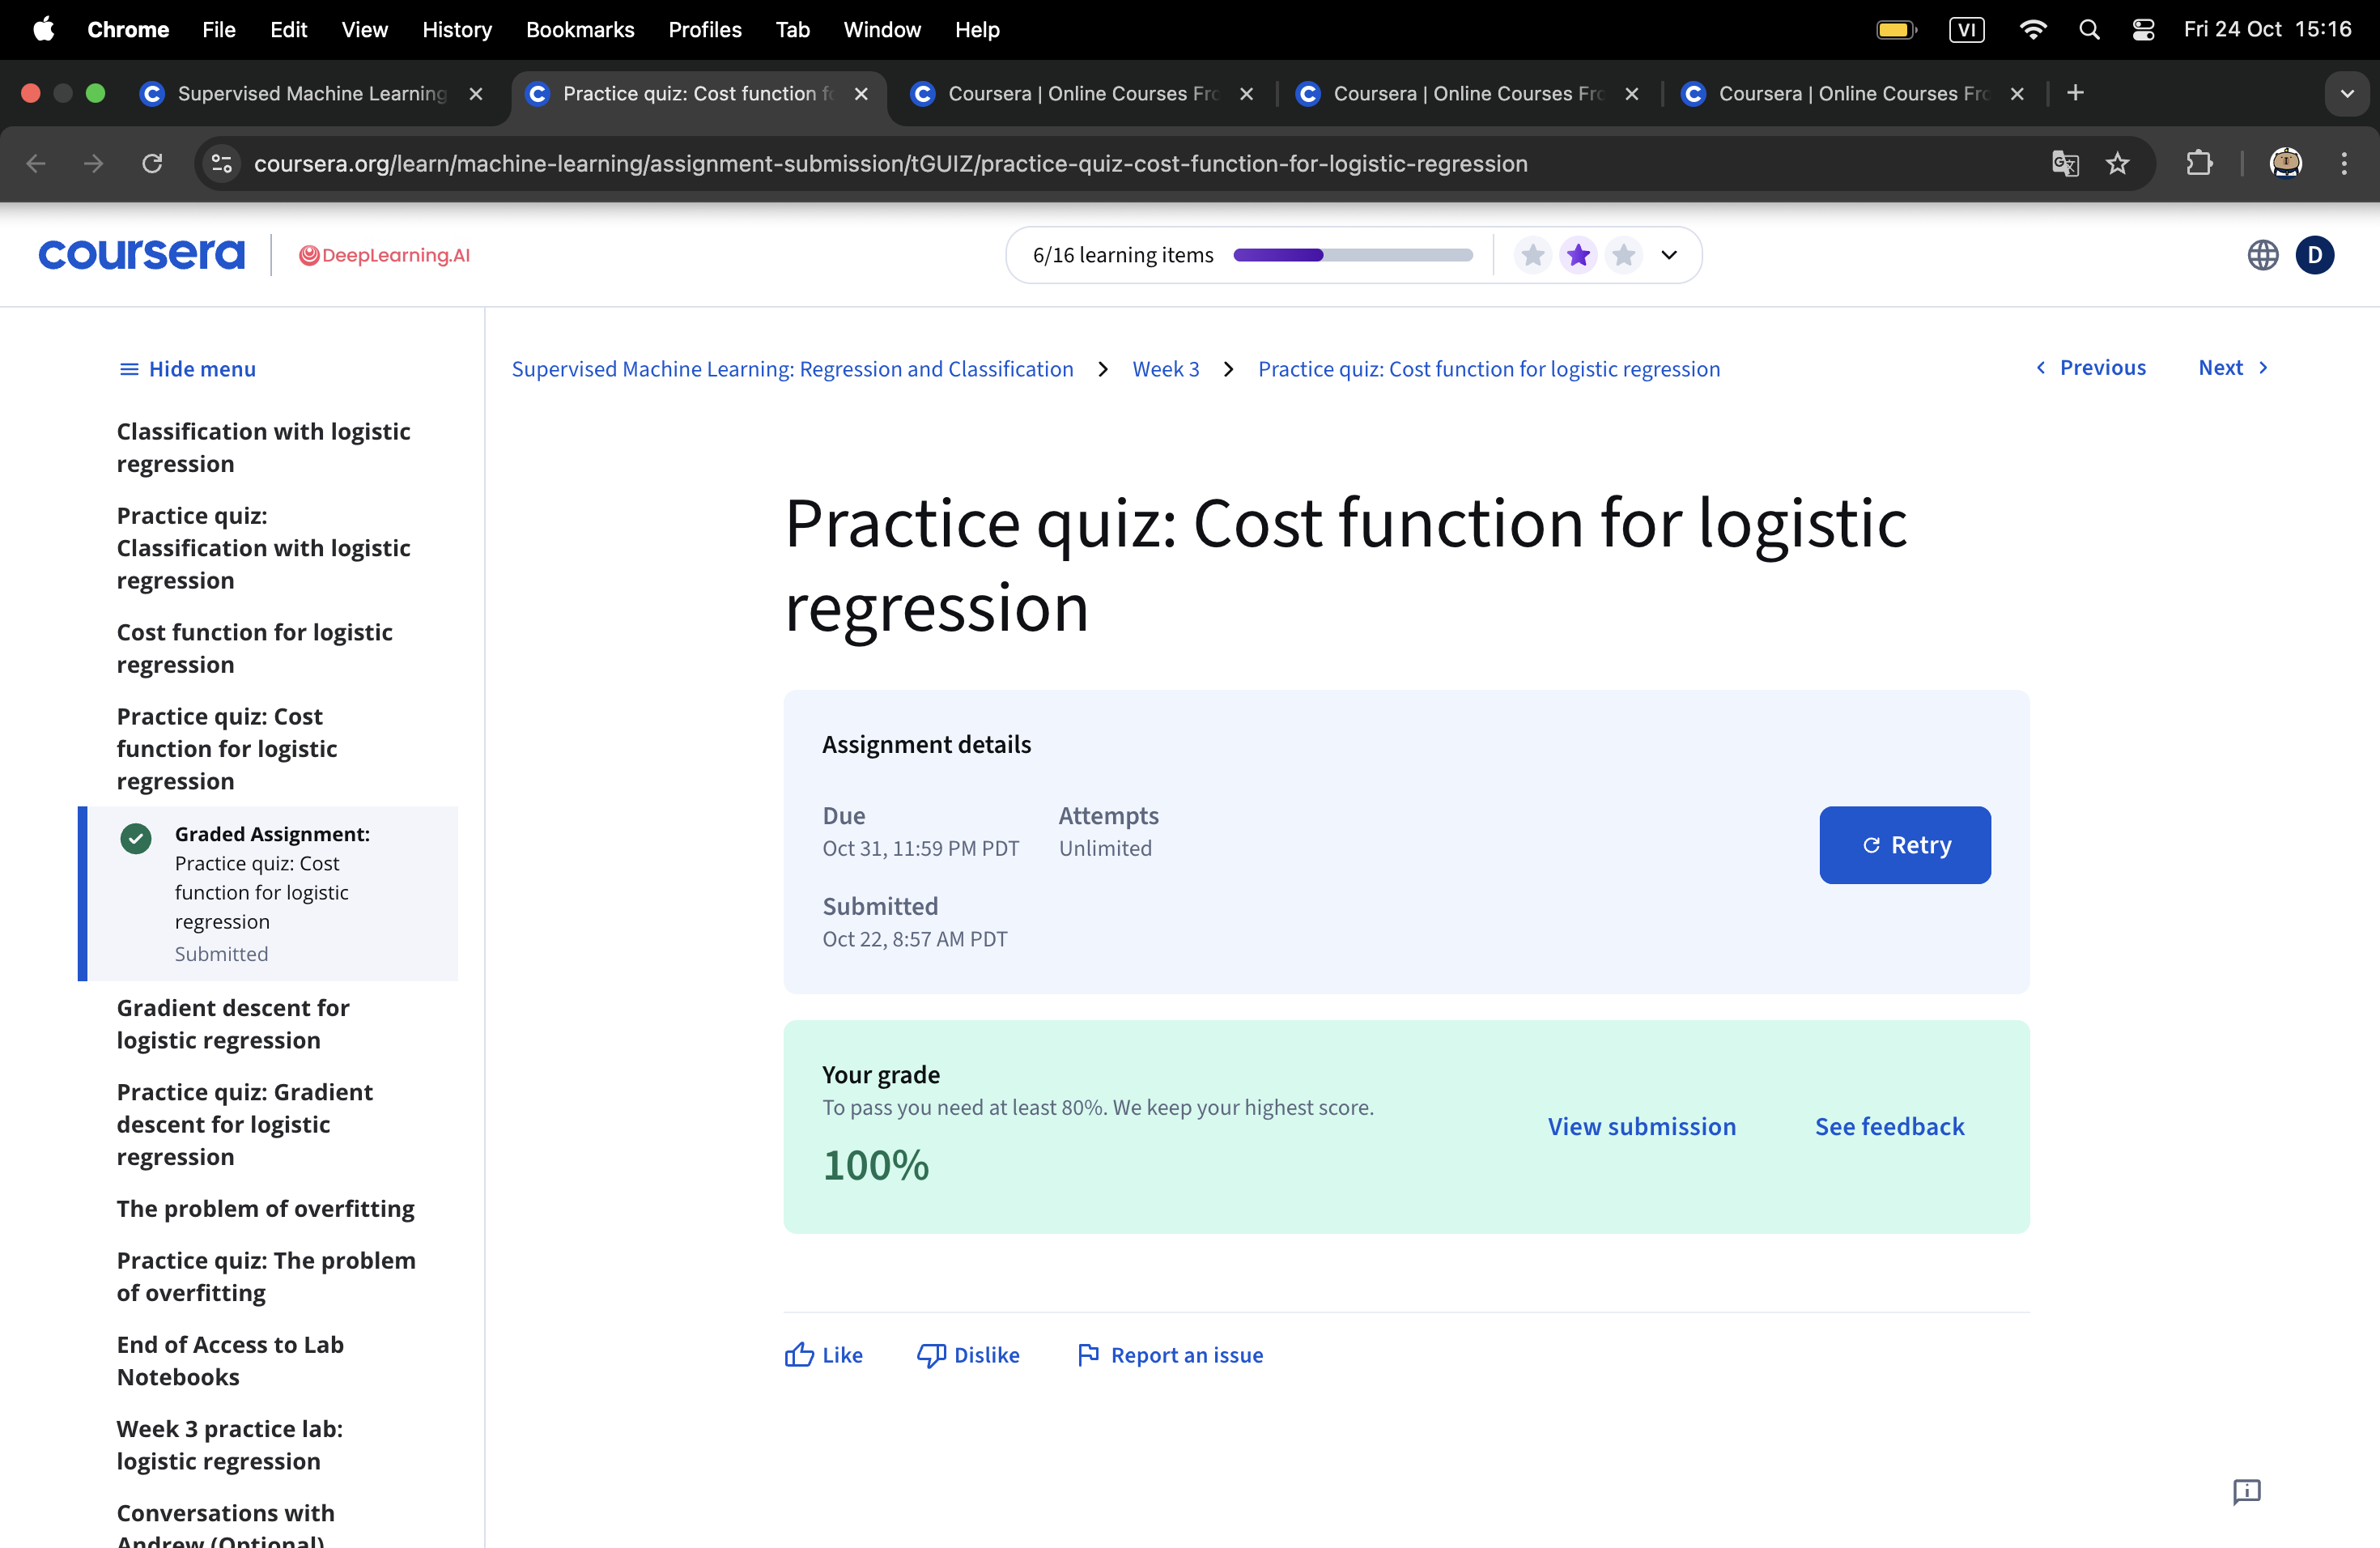
\includegraphics[scale=0.25]{Image/c1_w3_q2.png}
    \caption{Completed Graded Assignment 2 (Cost function for logistic regression)}
\end{figure}

\begin{figure}[H]
    \centering
    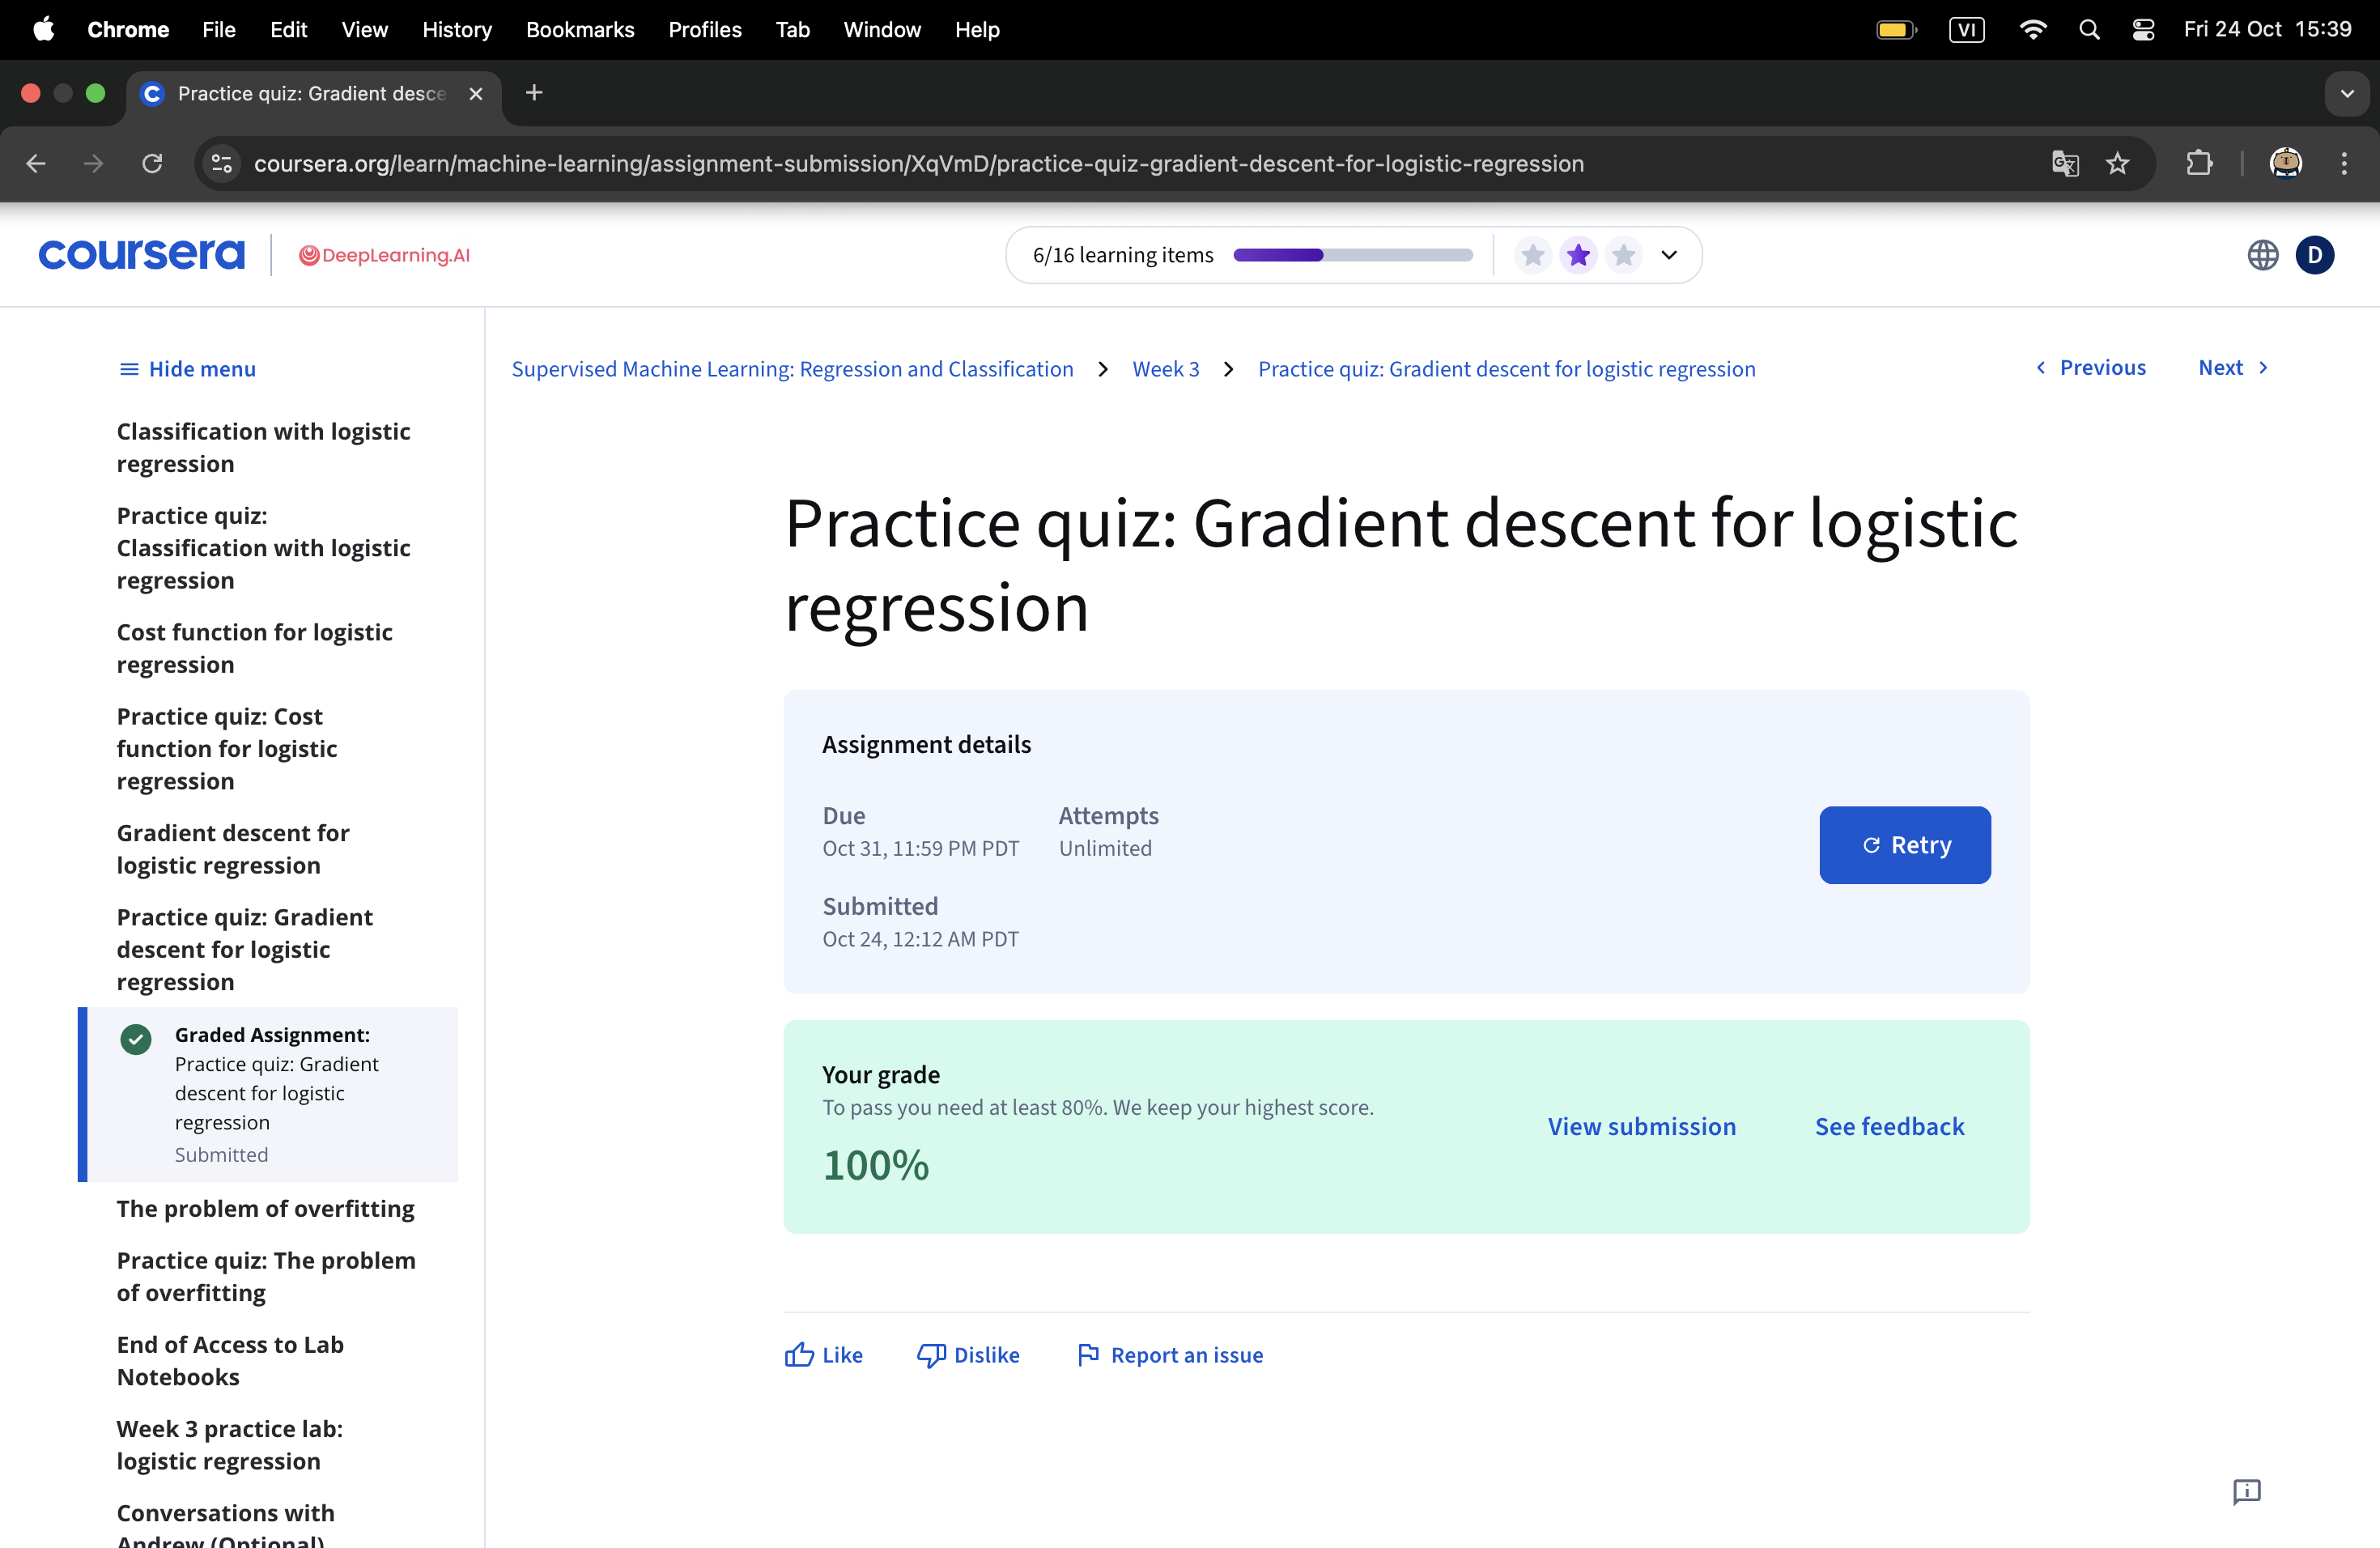
\includegraphics[scale=0.25]{Image/c1_w3_q3.png}
    \caption{Completed Graded Assignment 3 (Gradient descent for logistic regression)}
\end{figure}

\begin{figure}[H]
    \centering
    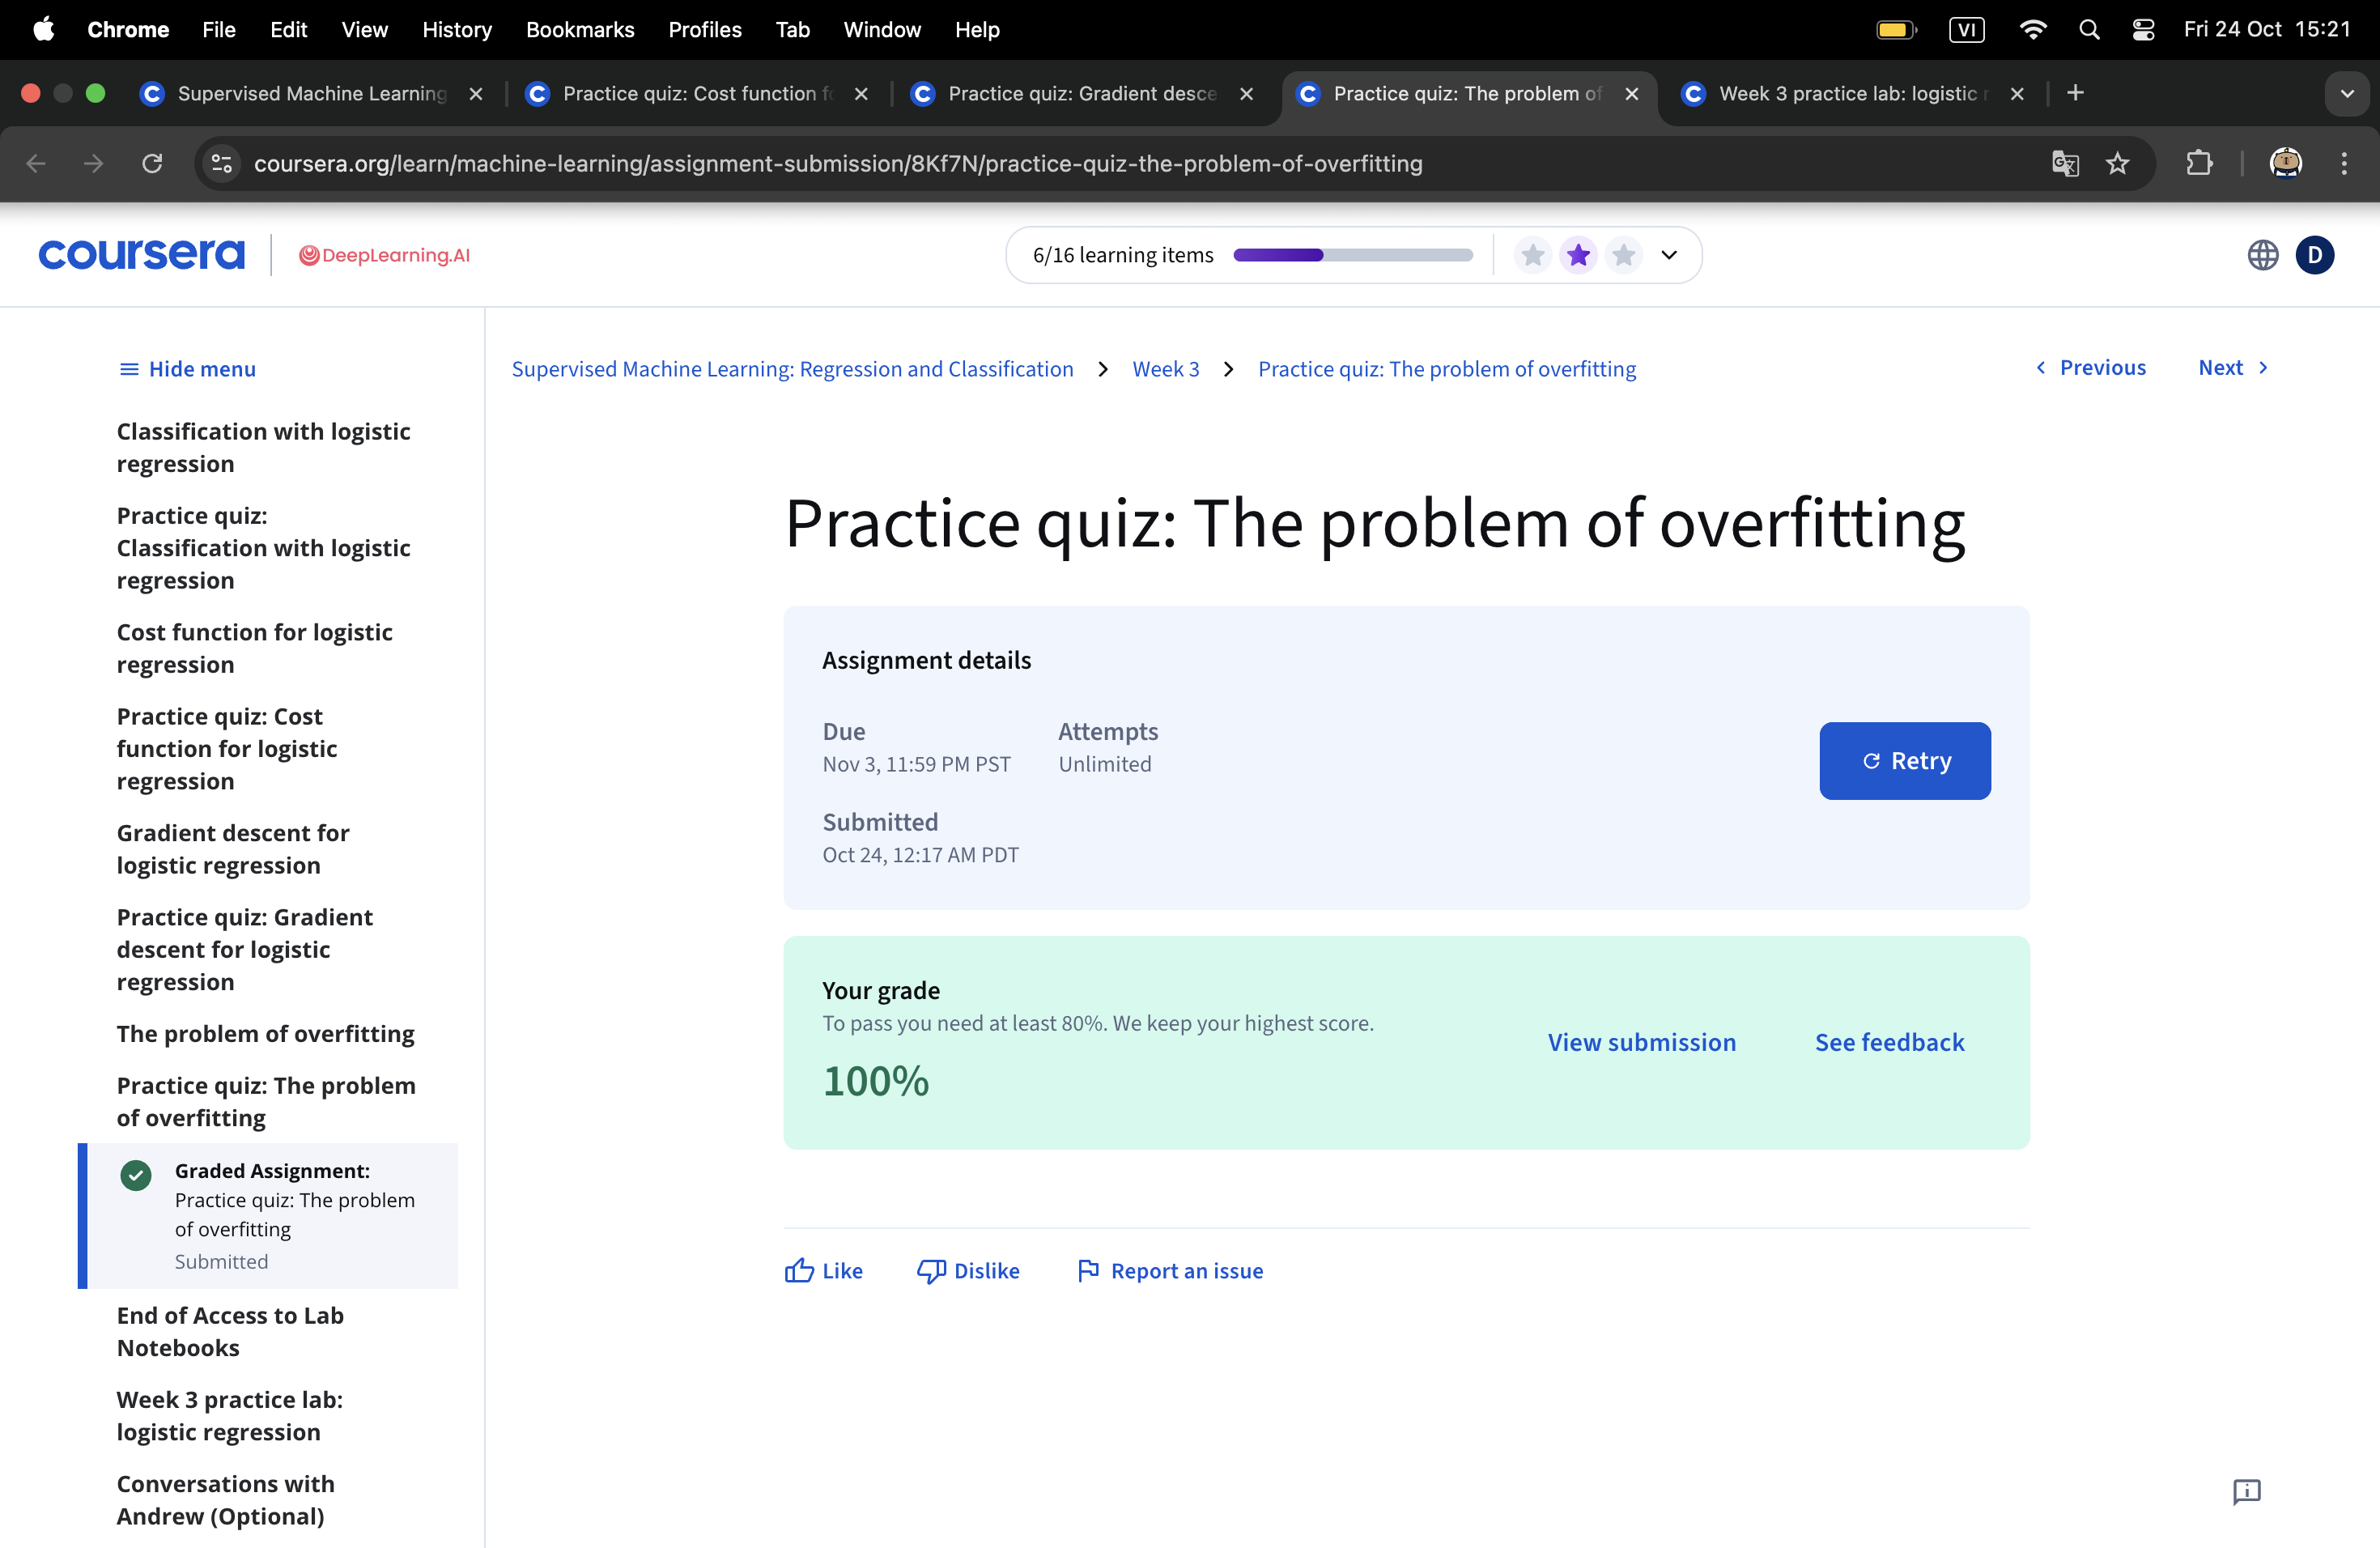
\includegraphics[scale=0.25]{Image/c1_w3_q4.png}
    \caption{Completed Graded Assignment 4 (The problem of overfitting)}
\end{figure}

\begin{figure}[H]
    \centering
    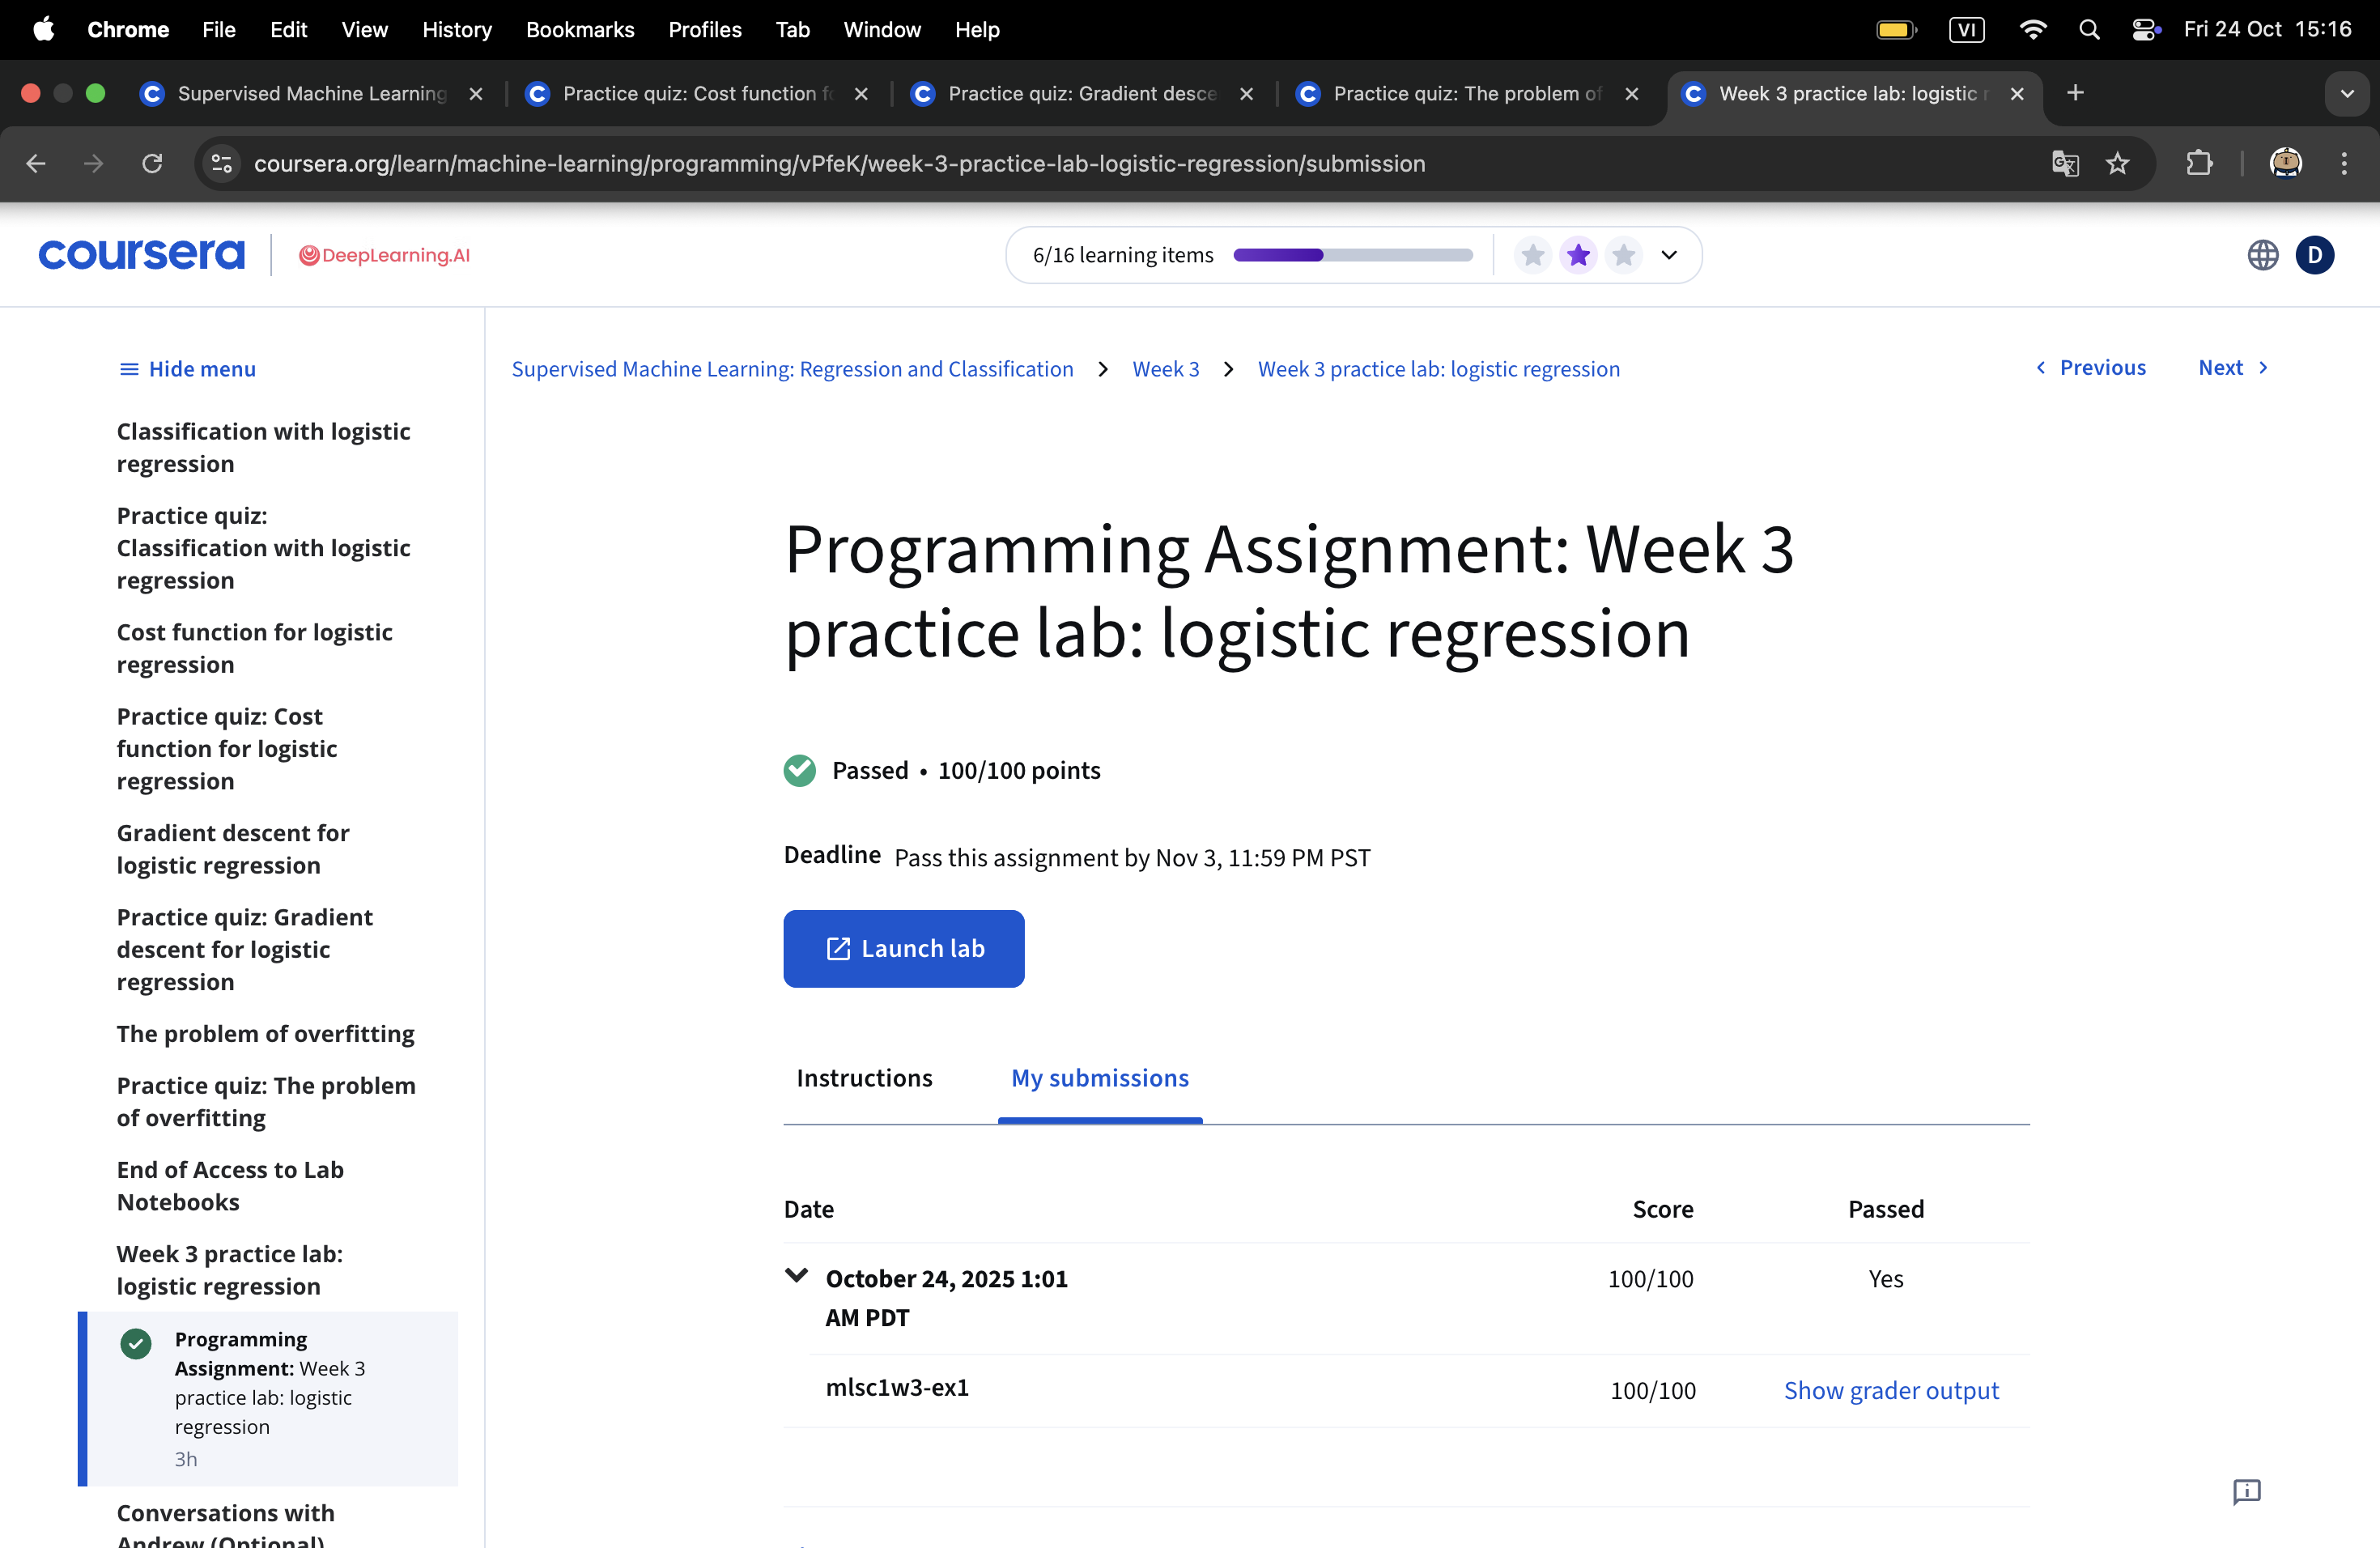
\includegraphics[scale=0.25]{Image/c1_w3_q5.png}
    \caption{Completed Programming Assignment (Logistic regression)}
\end{figure}

\subsection{Certificate for Completion}
\begin{figure}[H]
    \centering
    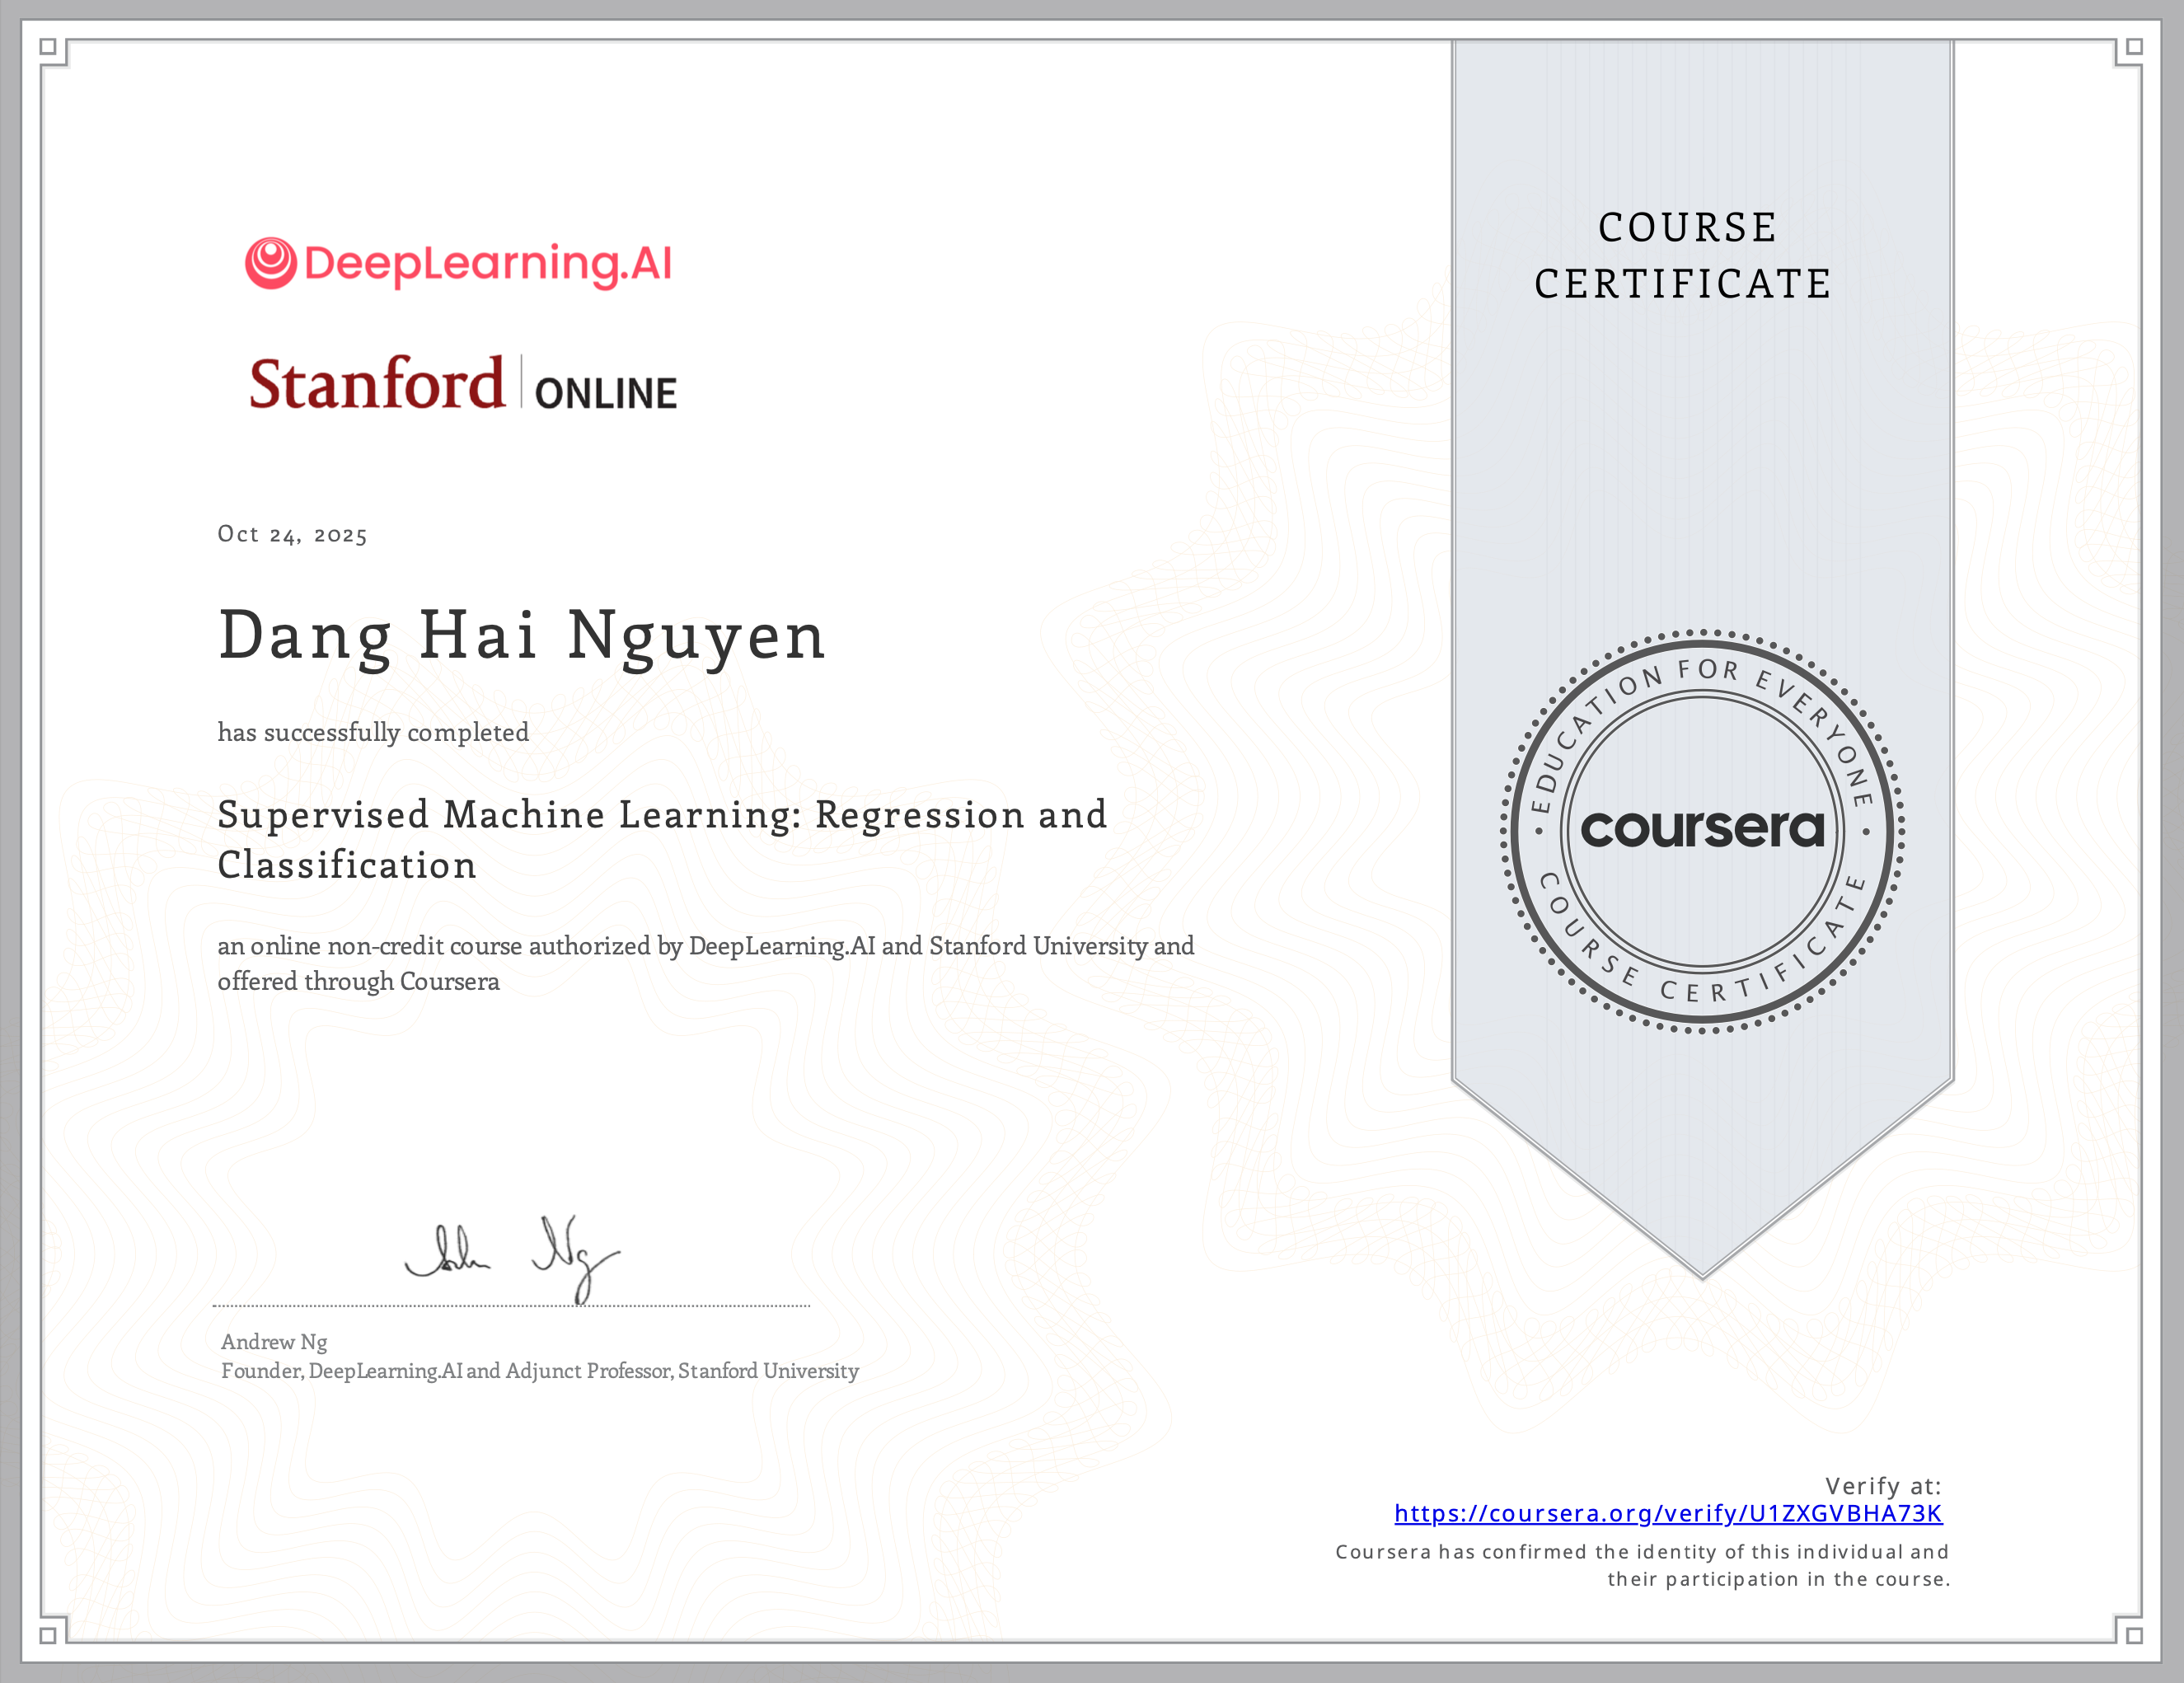
\includegraphics[scale=0.25]{Image/c1_certi.png}
    \caption{Certificate of completion for the course \textit{Supervised Machine Learning: Regression and Classification}.}
\end{figure}

